% To check for overfull hboxes, add draft to the document options
\documentclass[a4paper, 11pt]{report}
\usepackage[dutch]{babel}   % Taal van het document (opmaakregels ed.)
\usepackage{fancyhdr} % Fancy headers & footers

\usepackage{graphicx}
\usepackage{subfigure}	% Multiple figures in one float

\usepackage{color}
\usepackage{colortbl}	% Use colors in table
\usepackage{multirow}	% Multiple rows and columns in tables
\usepackage{booktabs}	% Professional looking tables

\usepackage{amsmath,amsfonts}    % Wiskunde

\usepackage{listings}            % Code Listings
%\usepackage[subfigure]{tocloft}		% Lijsten van willekeurige dingen + optie om errors met subfigure te vermijden
\usepackage[ruled,vlined,linesnumbered]{algorithm2e}	% Algorithm typesetting
%\usepackage{url}                % Opmaak van URLs

\usepackage{pdfpages}            % Maak dat voorblad kan toegevoegd worden
\usepackage[pdftex, pdfborder={0 0 0}]{hyperref}	% Links in pdf

\usepackage{ifthen}	% Conditionele stuff
\newboolean{makeall}	% Als dit true is, wordt inhoudsopgave etc toegevoegd
\newboolean{dankwoord}
\newboolean{spacepar}	% Spatie tussen paragrafen in plaats van indentatie
\setboolean{makeall}{true}
\setboolean{dankwoord}{false}
\setboolean{spacepar}{false}

\usepackage{tikz}	% Graphics framework
\usetikzlibrary{positioning}
\usetikzlibrary{calc}

% Karnaugh map macro
% Takes 5 arguments:
%	- Number of variables
%	- Function description (not used right now)
%	- Variable names, if the name is more than 1 char, enclose in {}
%	- Output values, if not 1 char, again enclose in {}
%	- Tikz functions (eg. for drawing rectangles around the minimizations)
%
% Furthermore, for ease of use, each point on the grid (where 2 lines meet) has a 
% named node attached to it, starting with G0 at the top left, G1 to the right of it, etc.
%
% Should it be required, the output values are named as well, starting with I0, I1, ...

% Argument string macro shamelessly stolen from Andreas W. Wielands Karnaugh map code
\def\kmapargumentstring#1{\gdef\kmapdummystring{#1{}\noexpand\end}}
\def\kmapgetchar{\expandafter\kmapgetonechar\kmapdummystring}
\def\kmapgetonechar#1#2\end{{#1}\gdef\kmapdummystring{#2\noexpand\end}}%

% Some counters
\newcounter{karnaughgrid}
\newcounter{karnaughindex}

\newcounter{karnaughsize}
\newcounter{karnaughsizex}
\newcounter{karnaughsizey}

\newcommand{\kmap}[5]{%
\setcounter{karnaughsize}{#1}

\begin{tikzpicture}
	\setcounter{karnaughgrid}{0};
	\setcounter{karnaughindex}{0};

	\ifcase\value{karnaughsize}
		% Size 0
		\exit
	\or
		% Size 1
		\setcounter{karnaughsizex}{2}
		\setcounter{karnaughsizey}{1}
	\or
		% Size 2
		\setcounter{karnaughsizex}{2};
		\setcounter{karnaughsizey}{2};
	\or
		% Size 3
		\setcounter{karnaughsizex}{4}
		\setcounter{karnaughsizey}{2}
	\or
		% Size 4
		\setcounter{karnaughsizex}{4}
		\setcounter{karnaughsizey}{4}
	\else
		\exit	% Wrong size
	\fi

	% Background grid
	\draw	(0,0) grid (\arabic{karnaughsizex},\arabic{karnaughsizey});

	% Set named node at each grid point for ease of drawing boxes & text later
	\foreach \y in {\arabic{karnaughsizey},...,0} {
		\foreach \x in {0,...,\arabic{karnaughsizex}} {
			\node (G\arabic{karnaughgrid}) at (\x, \y) {};
			\addtocounter{karnaughgrid}{1};
		}
	}

	% Draw function name
	\node at ($(G0) + {\value{karnaughsizey}/2}*(-0.4, 0) + {\value{karnaughsizex}/2}*(0, 0.4)$) [left] {#2};

	% Set bounding box to current size for nicer centering
	%\useasboundingbox;

	% Counting starts at 0, so lower size counters
	\addtocounter{karnaughsizex}{-1};
	\addtocounter{karnaughsizey}{-1};

	\kmapargumentstring{#4}

	\foreach \y in {\arabic{karnaughsizey},...,0} {
		\foreach \x in {0,...,\arabic{karnaughsizex}} {
			\node (I\arabic{karnaughindex}) at (\x, \y) [above right=-0.05 and -0.05] {\tiny \arabic{karnaughindex}};
			\addtocounter{karnaughindex}{1};

			\node at (\x + 0.5, \y + 0.5) {\large \kmapgetchar};
		}
	}

	% Draw variable names
	\kmapargumentstring{#3}

	\ifcase\value{karnaughsize}
		% No zero size maps
	\or
		% Size 1 maps
		\draw[arrows=|-|] ($(node cs:name=G1, anchor=north) + (0, 0.1)$) -- node[above] (V1) {\kmapgetchar} ($(node cs:name=G2, anchor=north)  + (0, 0.1)$);
	\or
		% Size 2 maps
		\draw[arrows=|-|] ($(node cs:name=G1, anchor=north) + (0, 0.1)$) -- node[above] (V1) {\kmapgetchar} ($(node cs:name=G2, anchor=north)  + (0, 0.1)$);
		\draw[arrows=|-|] ($(node cs:name=G3, anchor=west) + (-0.1, 0)$) -- node[left] (V2) {\kmapgetchar} ($(node cs:name=G6, anchor=west)  + (-0.1, 0)$);
	\or
		% Size 3 maps
		\draw[arrows=|-|] ($(node cs:name=G2, anchor=north) + (0, 0.8)$) -- node[above] (V1) {\kmapgetchar} ($(node cs:name=G4, anchor=north)  + (0, 0.8)$);
		\draw[arrows=|-|] ($(node cs:name=G5, anchor=west) + (-0.1, 0)$) -- node[left] (V2) {\kmapgetchar} ($(node cs:name=G10, anchor=west)  + (-0.1, 0)$);
	\draw[arrows=|-|] ($(node cs:name=G1, anchor=north) + (0, 0.1)$) -- node[above] (V3) {\kmapgetchar} ($(node cs:name=G3, anchor=north)  + (0, 0.1)$);
	\else
		% Size 4 maps
		\draw[arrows=|-|] ($(node cs:name=G10, anchor=west) + (-1, 0)$) -- node[left] (V1) {\kmapgetchar} ($(node cs:name=G20, anchor=west)  + (-1, 0)$);
		\draw[arrows=|-|] ($(node cs:name=G2, anchor=north) + (0, 0.8)$) -- node[above] (V2) {\kmapgetchar} ($(node cs:name=G4, anchor=north)  + (0, 0.8)$);
		\draw[arrows=|-|] ($(node cs:name=G5, anchor=west) + (-0.1, 0)$) -- node[left] (V3) {\kmapgetchar} ($(node cs:name=G15, anchor=west)  + (-0.1, 0)$);
		\draw[arrows=|-|] ($(node cs:name=G1, anchor=north) + (0, 0.1)$) -- node[above] (V4) {\kmapgetchar} ($(node cs:name=G3, anchor=north)  + (0, 0.1)$);
	\fi

	% Draw extra stuff (like minimizations)
	#5
\end{tikzpicture}}
	% Karnaugh map macros

%\usepackage{tikz}
%\pgfrealjobname{thesis}

% Lengtes
%\addtolength{\parskip}{10pt}
%\addtolength{\intextsep}{10pt}
%\addtolength{\belowcaptionskip}{-10pt}

% Hyphenation
%\hyphenation{}

% Math stuff
\newcommand{\xor}{\oplus}

% Citatie commando's
\newcommand{\reffig}[1]{Figuur~\ref{#1}}
\newcommand{\reftbl}[1]{Tabel~\ref{#1}}
\newcommand{\refalg}[1]{Algoritme~\ref{#1}}
\newcommand{\refsect}[1]{Paragraaf~\ref{#1}}
\newcommand{\refhfdst}[1]{Hoofdstuk~\ref{#1}}
\newcommand{\refform}[1]{Formule~\ref{#1}}

% Misc commando's
\newcommand{\nr}{n$^{\circ}$~}
%\def\@fnsymbol#1{\ifcase#1\or *\or \dagger\or \ddagger\or \mathchar "278\or \mathchar "27B\or \|\or **\or \dagger\dagger \or \ddagger\ddagger \else\@ctrerr\fi\relax}
\renewcommand{\thefootnote}{\fnsymbol{footnote}}	% Voetnoten met symbolen ipv nummers

% Narrow environment for wide tables & figures
% Usage: \begin{narrow}{-left cm}{-right cm}
\newenvironment{narrow}[2]{%
  \begin{list}{}{%
    \setlength{\topsep}{0pt}%
    \setlength{\leftmargin}{#1}%
    \setlength{\rightmargin}{#2}%
    \setlength{\listparindent}{\parindent}%
    \setlength{\itemindent}{\parindent}%
    \setlength{\parsep}{\parskip}%
  }%
  \item[]
}{\end{list}}

% List of equations
%\newcommand{\listequationsname}{List of vergelijkingen}
%\newlistof{myequations}{equ}{\listequationsname}
%\newcommand{\myequations}[1]{%
%\addcontentsline{equ}{myequations}{\protect\numberline{\theequation}#1}\par}

% BibTex opmaak
%\bibliographystyle{abbrvurl}
%\bibliographystyle{abbrv}
%\bibliographystyle{plain}
%\bibliographystyle{IEEEtranS} % Sorted IEEE style
\bibliographystyle{IEEEtran} % Unsorted IEEE style

% Fix for unsorted bibliographies & citations in captions
\def\@starttoc#1{%
  \begingroup
    \@fileswfalse
    \makeatletter
    \@input{\jobname.#1}%
  \endgroup
  \if@filesw
    \expandafter\newwrite\csname tf@#1\endcsname
    \immediate\openout \csname tf@#1\endcsname \jobname.#1\relax
  \fi
  \@nobreakfalse
}

% Substring macro
\def\substring#1#2#3{%
  \expandafter\subm\romannumeral#3000x.{}#1\relax\relax{#2}}
\def\subm#1#2.#3#4\relax#5\relax{%
  \csname sub#1\endcsname#2.#4\relax#5#3\relax}
\def\subx#1.#2\relax#3\relax#4{%
  \expandafter\submb\romannumeral#4000x.{}{}#3\relax}
\def\submb#1#2.#3{\csname sub#1b\endcsname#2.}
\def\subxb#1.#2\relax{#2}

% Plaats van afbeeldingen
\graphicspath{{images/}}
\DeclareGraphicsExtensions{.pdf,.eps,.png}

% Stel headers & footers in
\fancyhfoffset[EO]{2.5cm}

\fancyhead[LE, LO]{\small \slshape \rightmark}
\fancyhead[RE, RO]{\small \slshape \leftmark}

% Voor afwisselende pagina's:
%\fancyhead[LE,RO]{\small \slshape \rightmark}
%\fancyhead[RE,LO]{\small \slshape \leftmark}

\fancyfoot[CE,CO]{\thepage}

\pagestyle{fancy}

% Fix caption spacing bij tabellen
\setlength{\belowcaptionskip}{6pt}

% Zet hier de woorden waarmee de splitser problemen heeft:
\hyphenation{}

% Regel nummering van figuren
\renewcommand{\thefigure}{\thechapter.\arabic{figure}}
\newcommand{\Chapter}[1]{\chapter{#1} \setcounter{figure}{0}}

% Cell coloring
\newcommand{\shadecell}{\cellcolor{black!65}}

% Algorithm2e setup
\renewcommand{\listalgorithmcfname}{Lijst van algoritmes}
\renewcommand{\algorithmcfname}{Algoritme}
\renewcommand{\thealgocf}{\thechapter.\arabic{algocf}}
\SetCommentSty{textsf}
\SetKwComment{Comment}{}{}
\newcommand{\comm}[1]{\Comment*[f]{#1}}

% Listings setup
\definecolor{darkkeyword}{rgb}{0,0.08,0.40} %Requires the color package.
\definecolor{gray}{gray}{0.7}

\lstdefinelanguage{gezel}{
  tabsize=3,
  frame=single,
  basicstyle=\footnotesize\ttfamily,
  rulecolor=\color{gray},
  identifierstyle=, % nothing happens
  commentstyle=\color{gray}, % red comments
  stringstyle=\color{gray},%\ttfamily, % typewriter type for strings
  showstringspaces={false}, % no special string spaces
  morecomment=[l]{//},
  morestring=[b]",
  morekeywords={always, dp, in, out, tc, ns, reg, sig, sfg, hardwired, sequencer,
                fsm, use, ipblock, ipparm, iptype, lookup, initial, state, system,
                if, then, else, stimulus},
                keywordstyle=\color{blue}\bfseries,classoffset=1,
  morekeywords={\$display, \$cycle, \$dec, \$bin, \$dp, \$finish,
                \$hex, \$sfg, \$trace, \$option},
                keywordstyle=\color{darkkeyword}\bfseries,classoffset=0
}

\lstset{language=gezel,
        showstringspaces=false,
        frameround=ftft,
        captionpos=b,
        xleftmargin=-1cm,
        xrightmargin=-1cm,
        numbers=left,
        numberstyle=\tiny,
        stepnumber=5,
        numberfirstline=true,
        firstnumber=1
}

\renewcommand*\lstlistlistingname{Lijst van listings}

% Voorkom lelijke opmaak
%\clubpenalty=8000
%\widowpenalty=8000
%\displaywidowpenalty=8000

%\hyphenpenalty=5000
%\tolerance=1000

%%% Code voor figuren %%%
%%% Plaatst figuur op huidige plaats %%%
%
%\vspace{\textfloatsep}
%\begin{minipage}{\linewidth}
%    \begin{center}
%    \includegraphics[width=311px]{fig}
%    \figcaption{Figuur uitleg}\label{Figuur label}
%    \end{center}
%    \end{minipage}
%\vspace{\textfloatsep}

\begin{document}
\dontprintsemicolon   % Don't print ; after each line in algorithms
\selectlanguage{dutch}  % Set hyphenation patterns
\hyphenation{}

% Include gedeelte (begint op nieuwe pagina
% Indien gewoon invoegen op huidige plaats \input

\ifthenelse{\boolean{makeall}}%
{
\pagestyle{empty}
\pagenumbering{roman}

% Voeg voorblad toe

\includepdf{voorblad.pdf}

% Copyright
\section*{}
\thispagestyle{empty}

\vfill

\copyright~Copyright K.U.Leuven

\bigskip \noindent Zonder voorafgaande schriftelijke toestemming van zowel de promotor(en) als de auteur(s) is overnemen, kopi\"eren, gebruiken of realiseren van deze uitgave of gedeelten ervan verboden. 

\medskip \noindent Voor aanvragen tot, of informatie i.v.m.\ het overnemen en/of gebruik en/of realisatie van gedeelten uit deze publicatie, wend U tot de K.U.Leuven, Departement Elektrotechniek - ESAT, Kasteelpark Arenberg 10, B-3001 Heverlee (Belgi\"e). Telefoon +32-16~32~11~30 \& Fax.\ +32-16~32~19~86

\medskip \noindent Voorafgaande schriftelijke toestemming van de promotor(en) is eveneens vereist voor het aanwenden van de in dit afstudeerwerk beschreven (originele) methoden, producten, schakelingen en programma's voor industrieel of commercieel nut en voor de inzending van deze publicatie ter deelname aan wetenschappelijke prijzen of wedstrijden.

\bigskip
\bigskip
\bigskip

\noindent \copyright~Copyright by K.U.Leuven

\bigskip \noindent Without written permission of the promotors and the authors it is forbidden to reproduce or adapt in any form or by any means any part of this publication. 

\medskip \noindent Requests for obtaining the right to reproduce or utilize parts of this publication should be addressed to K.U.Leuven, Departement Elektrotechniek - ESAT, Kasteelpark Arenberg 10,  B‑3001 Heverlee  (Belgium). Tel.\ +32-16~32~11~30 \& Fax.\ +32-16~32~19~86.

\medskip \noindent A written permission of the promotor is also required to use the methods, products, schematics and programs described in this work for industrial or commercial use, and for submitting this publication to scientific contests.

\clearpage


\ifthenelse{\boolean{dankwoord}}{
\chapter*{Voorwoord}

Graag zou ik mijn promotoren Bart Preneel en Ingrid Verbauwhede bedanken voor het mogelijk maken van deze thesis. Indien zij er niet geweest waren, zou het nooit bij me opgekomen zijn een thesis over dit onderwerp te maken.

Verder wil ik graag mijn dagelijkse begeleiders Lejla Batina en \mbox{Miroslav} Knezevic bedanken voor hun steun en vele raad die ze mij gaven. Lelja wil ik specifiek bedanken voor de vele papers die ze mij bezorgde en haar hulp bij verscheidene wiskundige struikelblokken die ik tegenkwam. Miroslav dank ik voor zijn inzicht i.v.m.\ hardware en de vele tijd die hij stak in het helpen synthetiseren van mijn uiteindelijke ontwerp.

Ook dr.\ ir.\ Frederik Vercauteren verdient speciale vermelding. Zijn vermogen om de ingewikkelde wiskunde achter cryptografie zo uit te leggen dat zelfs een klein kind het nog zou begrijpen, heeft mij meer inzicht in de materie gegeven. Ook zijn hulp met bepaalde software en zijn niet aflatende vrolijkheid geappreci\"eerde ik ten zeerste.

Dr.\ ir.\ Nele Mentens verdient als nalezer ook een bedanking in dit voorwoord. Zonder haar kritisch oog was deze tekst vast en zeker niet geworden wat hij nu is.

Mijn vrienden wil ik graag bedanken voor hun steun en de vele fijne momenten die we samen beleefden dit jaar. Zonder hen zou het afgelopen jaar ongetwijfeld een stuk minder memorabel geweest zijn. Ook wil ik specifiek Mathias De Somere bedanken voor zijn hulp bij het oplossen van (zowat steeds compleet irrelevante) wiskundige problemen.

Ten slotte wil ik graag mijn ouders bedanken. Zij hebben het voor mij mogelijk gemaakt de studies Burgerlijk Ingenieur te ondernemen en zijn me gedurende die hele tijd steeds onvoorwaardelijk blijven steunen.

\bigskip \bigskip
{\raggedleft	% Lijn rechts uit
Anthony Van Herrewege\\
22 mei 2009\\
}
  % Dankwoord
}{}

\chapter*{Samenvatting}

In deze thesis wordt de berekening van de Tate paring onder de loep genomen. Een paring is een wiskundige constructie waarvan in 2001 ontdekt werd dat ze gebruikt kan worden voor het implementeren van identiteits-gebaseerde cryptografie.

Er wordt een compact hardware ontwerp voorgesteld dat de Tate paring over een supersinguliere kromme in $\mathbb{F}_{2^{163}}$ op een zeer zuinige manier kan berekenen. Het geheugengebruik van de ge\"implementeerde algoritmes wordt geminimaliseerd en een ontwerp voor een effici\"ent geheugenblok passeert de revue. Ook wordt het effect van verscheidene vermogensoptimalisaties onderzocht.

De uiteindelijke schakeling neemt minimum ongeveer 30k gates in beslag, dit is meer dan drie keer kleiner dan het kleinste ontwerp uit de literatuur. Een vermogenverbruik zo laag als 206 nanowatt kan bereikt worden, hoewel in dat geval de rekentijd 51,5 seconden bedraagt. Indien gewenst kan de berekening versneld worden door uitbreiding van de rekenkern. De energie-effici\"entie is, afhankelijk van gekozen parameters, tussen twee en twintig maal beter dan die van de enige andere implementatie uit de literatuur waarvoor dit berekend kon worden.

Ten tijde van dit schrijven zijn nog geen andere compacte, energie-effici\"ente ontwerpen gepubliceerd. Het voorgestelde ontwerp is in dat opzicht dus uniek.
 % Samenvatting

\tableofcontents
\clearpage

\listoffigures
\clearpage

\listoftables
\clearpage
  
\listofalgorithms
\clearpage

\chapter*{Lijst van afkortingen}

\begin{tabular}{l@{$\qquad$}l}
ASIC	& Application-Specific Integrated Circuit\\
ECC	& Elliptic Curve Cryptography\\
FPGA	& Field-Programmable Gate Array\\
MALU	& Modulaire Arithmetische Logische Unit\\
MUX	& Multiplexer\\
RAM	& Random-Access Memory\\
VHDL	& Very high speed integrated circuits Hardware Description Language\\
\end{tabular}
 % Lijst van afkortingen
\chapter*{Lijst van symbolen}

\section*{Algemeen}

\begin{tabular}{l@{$\qquad$}l}
$\mathbb{F}$	& Galois veld\\
$\mathbb{F}_q$	& Galois veld van $q$ elementen\\
$m$				& Graad van het Galois veld $\mathbb{F}_{2^m}$\\
$E$				& Elliptische kromme\\
$\#E$				& Aantaal punten op de elliptische kromme $E$\\
$x_A$				& x-co\"ordinaat van het punt $A$\\
$y_A$				& y-co\"ordinaat van het punt $A$\\
$e(P, Q)$		& Tate pairing van $P$ en $Q$\\
$A_i$				& Co\"efficient van graad $i$ van veelterm $A$ (tenzij expliciet anders vermeld)\\
$A_{i:j}$				& Co\"efficienten van graad $i$ t.e.m. $j$ van veelterm $A$\\
$\textsf{degree}(A)$	& Graad van de veelterm $A$\\
$\textsf{Hamm}(A)$	& Hamming gewicht van binaire representatie van $A$\\
$\textsf{min}(a, b)$	& Minimum  uit de lijst van opgegeven argumenten ($a$ en $b$)\\
$\textsf{rand}(E)$	& Willekeurig punt op de kromme $E$\\
\end{tabular}

\section*{Operators}

\begin{tabular}{l@{$\qquad$}l}
$\xor$	& exclusieve OR\\
$\#$		& concatenatie\\
$A \ll a$	& logische verschuiving van $A$ over $a$ posities naar links\\
$A \gg a$	& logische verschuiving van $A$ over $a$ posities naar rechts\\
$a \mid b$	& $a$ is een deler van $b$\\
\end{tabular}
    % Lijst van symbolen
}{}

\ifthenelse{\boolean{spacepar}}{
	% Paragraph spacing
	\setlength{\parindent}{0pt}
	\setlength{\parskip}{2ex plus 0.5ex minus 0.2ex}
}{}

\pagestyle{fancy}
\pagenumbering{arabic}

\Chapter{Inleiding}

 In dit inleidende hoofdstuk zal enige achtergrond informatie verschaft worden omtrent cryptografie. Verder wordt het concept identiteitsgebaseerde cryptografie duidelijk gemaakt. Er zal uitgelegd worden waarom de recente ondekking van pairings hier zo belangrijk voor is. Ten slotte geeft een kort overzicht aan wat in de literatuur terug te vinden is qua implementaties van pairings. In het volgende hoofdstuk wordt de werking van pairings dan wiskundig uitgespit.

\section{Basisachtergrond cryptografie}

Sinds het begin der tijden is er een nood geweest aan manieren om berichten versleuteld te verzenden tussen twee partijen. Voorbeelden van enkele klassieke encryptiemethoden zijn het Atbashcijfer~\cite{athbash} (Babyloni\"e, 600 v.\ Chr.), het Caesarcijfer~\cite{caesar} (Rome, 56 n.\ Chr.) en het dubbele transpositiecijfer~\cite{kahn} (o.a.\ gebruikt door weerstandsgroepen in WO II). E\'en eigenschap die al deze methodes met elkaar gemeen hebben, is het gebruik van dezelfde sleutel voor versleutelen en ontcijferen. Ook vele moderne encryptiemethodes, zoals bijvoorbeeld 3DES~\cite{3des} en AES~\cite{aes}, gebruiken dit principe, dat men symmetrische versleuteling noemt.

In \reffig{fig-encryptie-applicaties-sym-cipher} wordt de algemene werking van een symmetrische encryptie getoond. Alice zendt een bericht M naar Bob door het te versleutelen, vercijferd met een door hen beiden gekende sleutel $k$. Bob op zijn beurt ontcijfert met diezelfde sleutel de cijfertekst C. Indien Eve de vooraf afgesproken sleutel kent, kan zij alle communicatie tussen Alice en Bob ontcijferen. Er is dus nood aan een manier om veilig een sleutel $k$ te kunnen afspreken tussen twee partijen.

\begin{figure}[h]
	\centering
		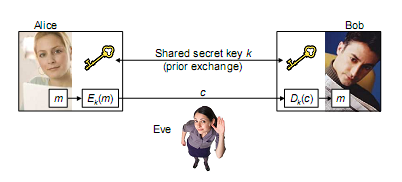
\includegraphics[scale=1.4]{symmetric-cipher-model}
		\caption{Algemene werking van symmetrische encryptie\label{fig-encryptie-applicaties-sym-cipher}}
\end{figure}

Een oplossing voor het veilig afspreken van een gedeelde sleutel was tot 1976 niet gekend. Toen stelden Diffie en Hellman hun algoritme voor sleuteluitwisseling over een onbeveiligd kanaal voor \cite{diffie-hellman}. Deze ontdekking plaveide de weg voor asymmetrische cryptografie (ook wel publieke sleutel cryptografie genoemd). Met behulp van dit type cryptografie kunnen eveneens boodschappen versleuteld worden. Dit wordt ge\"illustreerd in \reffig{fig-encryptie-applicaties-asym-cipher}. Wanneer Alice een bericht M naar Bob wil versturen, zoekt ze eerst zijn publieke sleutel $k_P$ op in een databank. Vervolgens versleutelt ze haar bericht met die publieke sleutel. Enkel Bob kan met behulp van zijn geheime sleutel $k_G$ dan het bericht ontcijferen. Een systeem als dit biedt het grote voordeel dat er geen nood is om de gebruikte (publieke) sleutel geheim te houden. Het is namelijk onmogelijk om met de publieke sleutel de cijfertekst te ontcijferen. Eve heeft er in dit geval dus geen baat bij de gebruikte publieke sleutel te onderscheppen. 

\begin{figure}[h]
	\centering
		 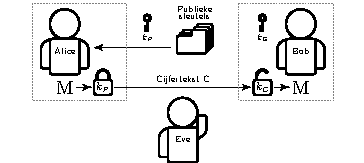
\includegraphics[scale=1.4]{asymmetric-cipher-model}
		 \caption{Algemene werking van asymmetrische encryptie\label{fig-encryptie-applicaties-asym-cipher}}
\end{figure}

Een andere toepassing van asymmetrische cryptografie is het plaatsen en verifi\"eren van digitale handtekeningen. Digitale handtekeningen zijn vergelijkbaar met klassieke handtekeningen. Ze kunnen, indien juist ge\-\"im\-ple\-men\-teerd, gebruikt worden om te verifi\"eren dat een bepaald bericht effectief door de persoon verstuurd is die de verzender beweert te zijn. Ook kan men aan de hand van een digitale handtekening nagaan of de inhoud van een bericht niet gewijzigd werd door een derde persoon tijdens de verzending. ECDSA \cite{ecdsa} en RSA \cite{rsa} zijn enkele van de vele cryptografische algoritmes die toelaten digitale handtekeningen te genereren.

Om te verzekeren dat de publieke sleutels van elke mogelijke ontvanger voorradig zijn, dient een soort een centrale databank voorzien te worden. Indien iemand het voor anderen mogelijk wil maken hem versleutelde berichten te versturen, genereert die persoon eerst een publieke en private sleutel. De publieke sleutel wordt vervolgens naar de database gestuurd, waar iedereen hem kan ophalen.

\section{Identiteitsgebaseerde cryptografie}

Een nadeel van de publieke sleutel cryptografie zoals voorgesteld in de vorige paragraaf zit hem in het sleutelbeheer. Er is geen manier om zeker te zijn dat wanneer de publieke sleutel van Bob opgevraagd wordt de verkregen sleutel effectief die van Bob is. Indien Eve bijvoorbeeld haar publieke sleutel in de database laat opslaan onder Bobs naam, zal Alice berichten voor Bob versleutelen met Eves publieke sleutel. Een mogelijke oplossing hiervoor is bijvoorbeeld het ``web of trust'', zoals ge\"implementeerd door de software PGP \cite{pgp}. Daarbij kunnen mensen aangeven of ze een bepaalde publieke sleutel betrouwbaar vinden of niet. Een sleutel die vergezeld wordt van meerdere getuigenissen van betrouwbaarheid zal dat dan waarschijnlijk ook zijn. Verder bestaat er een zogenaamde ``revocation list'', die aangeeft welke sleutels niet meer geldig zijn.

Uiteraard is ook zo een systeem niet volledig waterdicht. Iemand kan bijvoorbeeld onder verschillende identiteiten sleutels insturen en vervolgens met al die verschillende identiteiten zijn sleutels een certificaat van vertrouwen geven. Indien iemands publieke sleutel zou afgeleid kunnen worden van bekende gegevens omtrent zijn identiteit dan zouden deze problemen niet bestaan.

In 1984 stelde Shamir een methode voor waarbij dit mogelijk zou zijn \cite{shamir}. Het basisidee is als volgt: in plaats van een centrale databank voor publieke sleutels is er een centrale server die private sleutels voor elke gebruiker genereert aan de hand van geheime parameters. Gebruikers kunnen hun private sleutel dus niet zelf berekenen. De centrale server publiceert ook informatie omtrent hoe iemands identiteitsgegevens kunnen worden omgezet naar een publieke sleutel. Wanneer een gebruiker wil deelnemen aan beveiligde communicatie, meldt hij zich aan bij de centrale server en verkrijgt hij zijn private sleutel alsook de parameters om publieke sleutels te berekenen. Voor zowel de private sleutel als de parameters wordt er van uit gegaan dat deze levenslang gelden. Een gebruiker dient zich dus slechts \'e\'enmalig aan te melden.

Uiteraard is ook dit concept niet zonder problemen. Indien bijvoorbeeld de geheime parameters van de centrale server achterhaald worden, is het onmogelijk gebruikers daarvan op de hoogte te brengen. Een mogelijke oplossing is elke gebruiker om de zoveel tijd te voorzien van een nieuwe geheime sleutel. In dat geval stelt zich echter een nieuw probleem, want dan moet een methode bedacht worden om alle nieuwe sleutels bij de gebruikers te krijgen. 

Door deze problemen is de toepassing van identiteitsgebaseerde cryptografie eerder geschikt voor kleine groepen mensen, bijvoorbeeld intern in een bedrijf. In dat geval kost het weinig moeite iedereen op regelmatige tijdstippen van nieuwe sleutels te voorzien.

Een andere ideale toepassing is het gebruik van dit type cryptografie in netwerken van sensoren. Zo'n netwerk kan bestaan uit honderden nodes met een beperkte reken- en vermogenscapaciteit. Indien publieke sleutel cryptografie als vanouds zou worden gebruikt, zou dit leiden tot veel extra communicatie tussen de nodes en een centrale server. Telkens de nodes meetgegevens naar de server willen sturen, zouden ze diezelfde server eerst moeten contacteren om zijn publieke sleutel te weten te komen. In het omgekeerde geval zou de server telkens hij een node wil contacteren hetzelfde moeten doen.  Als echter identiteitsgebaseerde cryptografie wordt toegepast, is al die extra communicatie niet meer nodig, aangezien men de benodigde publieke sleutels kan berekenen met behulp van een unieke ID.

Een uitvoerig overzicht van identiteitsgebaseerde cryptografie en de bijhorende mogelijkheden en problemen valt buiten het bestek van thesis. In het volgende hoofdstuk zullen wel enkele mogelijkheden naderbij bestudeerd worden. Een uitstekend startpunt voor meer informatie is \cite{maas}.

\section{Pairings\label{inleiding-pairings}}

Hoewel het idee reeds in 1984 gepubliceerd werd, zou het echter tot 2001 duren eer Boneh en Franklin een effici\"ent algoritme voor identiteitsgebaseerde cryptografie voorstelden \cite{boneh}. Zij stelden een schema op dat toeliet de idee\"en van Shamir ook effectief te implementeren. In hun voorstel maakten ze gebruik van de Weil pairing \cite{weil}. Al gauw verschenen er variaties op het oorspronkelijke schema. Daarin werd het gebruik van andere pairings voorgesteld, zoals bijvoorbeeld de Tate \cite{tate} of de $\eta_T$ \cite{eta} pairing. Wat pairings juist zijn en hoe ze gebruikt kunnen worden, zal in het volgende hoofdstuk uitvoerig aan bod komen.

Alvorens de wiskunde achter pairings in te duiken, wordt eerst nog een overzicht gegeven van de huidige ``state of the art'' van implementaties van pairings. De mogelijkheden van implementaties op een microchip en een FPGA passeren de revue. Implementaties van pairings op computers zijn per definitie niet in een omgeving met beperkte ressources toepasbaar. Ze hebben dus weinig te maken met deze thesis, die als uitgangspunt compacte implementaties heeft. Vandaar dat dit type implementaties dan ook niet bestudeerd zal worden.

\subsection{Microchip implementaties}

Implementaties van pairings voor gebruik op een MICA node \cite{mica}, specifiek ontwikkeld voor gebruik in netwerken van sensoren, worden voorgesteld in \cite{tinytate}, \cite{tinypbc} en \cite{nanoecc}. De processor op deze node is een ATMega128L microchip \cite{atmega}. Een overzicht van de resultaten is gegeven in \reftbl{tabel-resultaten-sensor}. Rekening houdend met het stroomverbruik en de batterijspanning gegeven in \cite{nanoecc}, is het vermogenverbruik waarschijnlijk ongeveer $23.60$ $mW$.

\begin{table}[h]
	\caption[Resultaten uit de literatuur voor implementaties ontwikkeld op een MICA node]{Resultaten uit de literatuur voor implementaties ontwikkeld op een MICA node \cite{mica}}
	\label{tabel-resultaten-sensor}

	\centering
	\begin{tabular}{lllll}
		\toprule
		& \multirow{2}{*}{TinyTate \cite{tinytate}}	& \multirow{2}{*}{TinyPBC \cite{tinypbc}} &	\multicolumn{2}{c}{NanoECC \cite{nanoecc}}\\
		\cmidrule{4-5}
		& & & \multicolumn{1}{c}{Binair} & \multicolumn{1}{c}{Priem}\\
			\midrule
		Veld					& $\mathbb{F}_{p}$ 256 bit	& $\mathbb{F}_{2^{271}}$	& $\mathbb{F}_{2^{163}}$	& $\mathbb{F}_{p}$ 160 bit\\
		Pairing				& Tate							& $\eta_T$ 						& Tate							& Tate\\
		Rekentijd ($s$)	& 30.21							& 5.45							& 10.96							& 17.93\\
		\bottomrule
	\end{tabular}
\end{table}

\subsection{FPGA implementaties}

In de literatuur zijn vrij veel ontwerpen voor FPGA's terug te vinden. Het probleem is echter dat men zich bij het ontwerp hiervan steeds toelegt op het behalen van een zo hoog mogelijke snelheid, wat resulteert in een grote oppervlakte. Dit type implementaties is dus minder geschikt zijn voor toepassingen met beperkte ressources.

Toch wordt in \reftbl{tabel-resultaten-fpga} een sumier overzicht gegeven van een zeer beperkt aantal ontwerpen. Bij de selectie hiervan werd vooral gekozen voor ontwerpen waarin in een vrij klein veld gerekend werd. Er dient in acht te worden genomen dat bij al deze implementaties snelheid, en niet een compacte, zuinige implementatie, het voornaamste doel is. 

\begin{table}[h]
	\caption{Resultaten uit de literatuur voor implementaties ontwikkeld voor FPGA's}
	\label{tabel-resultaten-fpga}

	\centering
	\begin{tabular}{llllll}
		\toprule
		&	\multicolumn{1}{c}{Veld}	& \multicolumn{1}{c}{Pairing}	& $\begin{array}{@{}c@{}}\text{Opp.}\\\text{[slices]}\end{array}$	& $\begin{array}{@{}c@{}}f\\\text{[MHz]}\end{array}$	& $\begin{array}{@{}c@{}}\text{Reken-}\\\text{tijd }[\mu s]\end{array}$\\
		\midrule
		Ronan \emph{et al.} \cite{ronan}				& $\mathbb{F}_{2^{103}}$	& Tate		& 21021	& 51	& 206\\
		Shu \emph{et al.} \cite{shu}					& $\mathbb{F}_{2^{239}}$	& Tate		& 25287	& 84	& 41\\
		Keller \emph{et al.} \cite{keller}			& $\mathbb{F}_{2^{251}}$	& Tate		& 27725	& 40	& 2370\\
		Grabher en Page \cite{grabher}				& $\mathbb{F}_{3^{97}}$		& Tate		& 4481	& 150	& 432\\
		Beuchat \emph{et al.} \cite{beuchat-eta}	& $\mathbb{F}_{3^{97}}$		& $\eta_T$	& 1833	& 145	& 192\\
		\bottomrule
	\end{tabular}
\end{table}

       % Inleiding & motivatie

\Chapter{Pairings}

In dit hoofdstuk zal de werking van pairings wiskundig uit de doeken gedaan worden. Meer specifiek zal de Tate pairing bestudeerd worden. Er zal duidelijk gemaakt worden hoe de pairing berekend kan worden. Vervolgens worden enkele schema's voorgesteld die gebruikt kunnen worden voor versleuteling van gegevens en de aanmaak van digitale handtekeningen. In het volgende hoofdstuk wordt dan een schakeling ontworpen waarmee de Tate pairing berekend kan worden.

Enkel de hoogstnodige theorie zal hier behandeld worden. Voor een meer diepgaande uiteenzetting wordt opnieuw verwezen naar \cite{maas}. Het is ook uit dit werk dat de informatie uit de volgende paragrafen afkomstig is, tenzij anders vermeld.

\section{Inleidende wiskunde}

Alvorens de wiskundige theorie van pairings uit de doeken gedaan kan worden, dient die van elliptische krommen duidelijk gemaakt te worden. Het is met behulp van deze constructies dat pairings berekend kunnen worden. Elliptische krommen worden doorgaans echter gedefinieerd over een eindig veld. Vandaar dat de noodzakelijk theorie van beiden hier even heel kort herhaald wordt.

\subsection{Eindige velden}

Een eindig veld $\mathbb{F}_q$ wordt gedefinieerd door zijn karakteristiek $q$. Die karakteristiek is bij cryptografische toepassingen doorgaans een groot priemgetal $p$ of 2, hoewel tegenwoordig ook onderzoek gedaan wordt naar toepassingen met een karakteristiek 3. Een veld zonder zijn nul element wordt aangeduid als
\[\mathbb{F}_q^* = \mathbb{F}_q / \{ 0 \}.\]

Volgens de kleine stelling van Fermat geldt in elk eindig veld $a^q = a$. Van deze gelijkheid zal in het volgende hoofdstuk handig gebruikt gemaakt worden wanneer de inverse van een element moet berekend worden. Het voordeel van werken in een binair veld, m.a.w.\ $q = 2$, is dat optellingen en aftrekkingen equivalent zijn en zeer makkelijk uit te voeren zijn. Het is immers zo dat $1 + 1 = 2 \bmod 2 = 0$ en $0 - 1 = -1 \bmod 2 = 1$. Beiden kunnen dus berekend worden via een XOR operatie.

Verder kunnen extensies van graad $m$ van een veld gedefinieerd worden. In het geval $q = 2$ bekomt men dan een nieuw veld $\mathbb{F}_{2^m}$. Er dient dan ook een reductie veelterm $P$ opgegeven te worden. Een extensieveld wordt gedefinieerd als:
\[\mathbb{F}_{q^m} \cong \mathbb{F}_q [z] / (P). \]

\paragraph{Voorbeeld} Om de constructie van een extensieveld enigszins te verduidelijken wordt een klein voorbeeld gegeven. Er wordt gewerkt in karakteristiek $q = 2$. Stel $P = z^2 + z + 1$. Het extensieveld is dus gedefinieerd als:
\[\mathbb{F}_{2^2} \cong \mathbb{F}_2 [z] / (z^2 + z + 1). \]
Verder $A = z$ en $B = z + 1$. De resultaten van de optelling en vermenigvuldiging van $A$ en $B$ zijn dan respectievelijk:
\[\begin{aligned}
A + B &= 2z + 1 \qquad & A \cdot B &= z^2 + z\\
&= 1	& &= 2z + 1\\
\end{aligned}\]

\subsection{Elliptische krommen}

Een elliptische kromme $E$ wordt gevormd door de verzameling van punten die voldoen aan de vergelijking:
\[E: Y^2 Z + a_1 XYZ + a_2 Y Z^2 = X^3 + a_3 X^2 Z + a_4 X Z^2 + a_5 Z^3.\]
Het enige punt waarvoor $Z = 0$ en de vergelijking geldt ($X = 0,  Y = 1, Z = 0$), wordt het punt op oneindig $\mathcal{O}$ genoemd. Indien wordt gesteld dat $x = \frac{X}{Z}$ en $y = \frac{Y}{Z}$, bekomt men de affiene Weierstrass vergelijking:
\[E: y^2 + a_1 xy + a_2 y = x^3 + a_3 x^2 + a_4 x + a_5.\]
Merk op dat in deze vorm het punt $\mathcal{O}$ niet meer voldoet aan de vergelijking, ook al behoort het nog steeds tot de kromme. De kromme dient zo gedefinieerd te zijn dat $\forall A \in E$ de parti\"ele afgeleiden $\frac{\partial P}{\partial X}$, $\frac{\partial P}{\partial Y}$ en $\frac{\partial P}{\partial Z}$ nooit allen tegelijkertijd gelijk zijn aan nul.

De natuurlijke bewerking op een kromme is de ``tangent-and-chord'' methode, die wordt weergegeven in \reffig{figuur-pairings-tangent-and-chord}. De bewerking wordt additief geschreven en heeft als neutral element het punt op oneindig $\mathcal{O}$. Afhankelijk van het veld waarover de kromme gedefinieerd is, zullen de formules om de ``tangent-and-chord'' methode uit te voeren anders zijn. 

\begin{figure}[h]
	\centering
		\includegraphics[width=8cm]{tangent-and-add}
		\caption{``tangent-and-add'' methode op een elliptische kromme\label{figuur-pairings-tangent-and-chord}}
\end{figure}

Aan de hand van de vorige bewerking kan een scalaire vermenigvuldiging vastgelegd worden, met $a \in \mathbb{Z}$:
\[\begin{aligned}
a \cdot A	&= A + \ldots + A\\
0 \cdot A	&= \mathcal{O}\\
-a \cdot A	&= a \cdot -A
\end{aligned}\]

De orde $o$ van een punt $A$ op de kromme is gelijk aan de minimum waarde waarvoor $o \cdot A = \mathcal{O}$. Het is mogelijk dat $o = \infty$. Van alle punten waarvoor $o$ een deler is van $n$ wordt gezegd dat ze in de $n$-torsiesubgroep van $E$ zitten. Zo een subgroep wordt genoteerd als:
\[E[n] = \{ A \in E : n \cdot A = \mathcal{O} \}.\]

Het aantal punten $\#E$ op $E$ wordt de orde van de kromme genoemd. Voor een kromme over een veld $\mathbb{F}_q$ is $\#E = q + 1 - t$, met $t$ de ``trace'' van de kromme. Indien $q \mid t$ wordt de kromme supersingulier genoemd. Voor bepaalde types krommen bestaat er een gesloten formule voor $\#E$.

Ten slotte wordt nog de inbeddingsgraad $k$ gedefinieerd als het kleinste gehele getal waarvoor $n \mid q^k - 1$.

\section{Definitie van pairings}

Een pairing is in dit geval een functie $f(A, B)$ met als argumenten twee punten uit een additieve groep en als resultaat een punt in een multiplicatieve groep:
\[f(A, B): \mathbb{G}_1 \times \mathbb{G}_2 \rightarrow \mathbb{G}_T.\]
Een pairing moet tevens volgende eigenschappen bezitten: bilineariteit, non-degeneratie en moet goed gedefinieerd zijn. De betekenis van deze drie begrippen is:

\begin{enumerate}
	\item Bilineariteit: $\forall A_1, A_2, A \in \mathbb{G}_1$ en $\forall B_1, B_2, B \in \mathbb{G}_2$ geldt $f(A_1 + A_2, B) \equiv f(A_1, B) \cdot f(A_2, B)$ en $f(A, B_1 + B_2) \equiv f(A, B_1) \cdot f(A, B_2)$.

	\item Non-degeneratief: $\forall A \in \mathbb{G}_1, \: \exists B \in \mathbb{G}_2$ waarvoor $f(A, B) \neq 1$.

	\item Goed gedefinieerd: $\forall B \in \mathbb{G}_2$ is $f(A, B) = 1$ als en slechts als $A = \mathcal{O}$.
\end{enumerate}

Het zijn de drie eigenschappen waaraan pairings moeten voldoen die het zo moeilijk maken ze te genereren. Ten tijde van dit schrijven waren onder meer volgende pairings bekend: Weil, Tate, $\eta_T$ \cite{eta} en Ate \cite{ate}. In deze thesis zal gewerkt worden met de Tate pairing, waarvan bewezen is dat ze effici\"enter te berekenen is dan de Weil pairing.

De vermelde $\eta_T$ en Ate pairing zijn variaties op de Tate pairing die gebruikt kunnen worden indien voor specifieke elliptische krommen gekozen wordt. Indien aan de juiste voorwaarden voldaan wordt, zal de schakeling die in het volgende hoofdstuk wordt voorgesteld dus ook gebruikt kunnen worden om deze pairings te berekenen.

De definitie van de Tate pairing over elliptische krommen is als volgt:
\[e(A, B): E(\mathbb{F}_{q^k})[n] \times E(\mathbb{F}_{q^k})/n \cdot E(\mathbb{F}_{q^k}) \rightarrow \mathbb{F}_{q^k}^* / (\mathbb{F}_{q^k}^*)^n\]
Het resultaat van de Tate pairing is niet uniek, maar een element van een equivalentieklasse in $\mathbb{F}_{q^k}^* / (\mathbb{F}_{q^k}^*)^n$. Voor twee resultaten $a, b \in \mathbb{F}_{q^k}^*$ geldt $a \equiv b$ als en slechts als er een element $c \in \mathbb{F}_{q^k}^*$ waarvoor $a = bc^n$. Aangezien voor cryptografische toepassingen een uniek resultaat gewenst zal zijn, dient die $n$-de macht weggewerkt te worden. Dit kan door het resultaat te verheffen tot de macht $\frac{q^k - 1 }{n}$. Aangezien $a^{q^k - 1} = 1$ voor elke $a \in \mathbb{F}_{q^k}^*$ (kleine stelling van Fermat), verkrijgt men dan dus een $n$-eenheidswortel.

\section{Berekening van de Tate pairing}

Reeds in 1986 stelde Miller een methode voor om de Tate pairing te berekenen \cite{miller, barreto-efficient}. \refalg{algoritme-pairings-miller} geeft weer hoe dat algoritme  in z'n werk gaat.
        % Wiskundige informatie over pairings 

\Chapter{Implementatie\label{hfdst-implementatie}}

In dit hoofdstuk wordt de implementatie van een schakeling voor de berekening van de Tate pairing uit de doeken gedaan. Het uiteindelijke doel is een zo compact mogelijke  ASIC implementatie te verkrijgen.

Er zal onderzocht worden welke basisbewerkingen nodig zijn en hoe deze verwezenlijkt kunnen worden in hardware. Vervolgens wordt een schakeling ontworpen die aan de hand hiervan alle nodige berekeningen kan uitvoeren in het gekozen veld. Ten slotte is er dan nog de schakeling die alle berekeningen voor het Miller algoritme (zie \refsect{sectie-pairings-berekening}) in goede banen leidt. In het volgende hoofdstuk zal de resulterende schakeling dan beoordeeld worden.

Allereerst worden echter noodzakelijke parameters vastgelegd, zodat alle bewerkingen exact gedefini\"eerd kunnen worden. Vervolgens wordt bekeken welke beperkingen aan de schakeling opgelegd moeten worden.

\section{Parameters\label{sectie-implementatie-parameters}}

Alvorens kan begonnen worden met de implementatie, moeten bepaalde parameters vastgelegd worden. Pas eens dat gedaan is, zijn alle bewerkingen volledig gedefinieerd.

Een belangrijke parameter is het veld waarover gewerkt zal worden. Omdat de berekeningen in een veld $\mathbb{F}_2$ (en extensies ervan) veel eenvoudiger zijn dan die in een veld modulo een priemgetal, wordt ervoor gekozen in zulk een veld te werken.

Ook moet een kromme vastgelegd worden. Er wordt gekozen voor de reeds eerder vermelde supersinguliere elliptische kromme
\[E(\mathbb{F}_{2^m}): y^3 + y = x^3 + x + b,\]
waarbij $b \in \{0, 1\}$.  Dat type krommen heeft een kleine inbeddingsgraad $k = 4$ en geeft aanleiding tot simpele rekenregels voor de verdubbeling en optelling van punten \cite{barreto-efficient, hankerson-book}. Verder worden de volgende hulp variabelen bepaald:
\[\begin{aligned}
\delta	&= b	\qquad	& m \equiv 1, 7 \quad(\bmod \; 8)\\
			&= 1 - b		& m \equiv 3, 5 \quad(\bmod \; 8)\\
\nu		&= (-1)^{\delta}\\
\end{aligned}\]
De orde van de kromme is gelijk aan \cite{bertoni, beuchat}:
\[\begin{aligned}
\#E(\mathbb{F}_{2^m})	&= 2^m + \nu \sqrt{2^{m + 1}} + 1
\end{aligned}\]
Om de Tate pairing te kunnen berekenen, moet de variabele $b$ zo gekozen worden dat $\#E$ enkel uit optellingen bestaat. Met andere woorden: $b$ moet zo gekozen worden dat $\nu = 1$.

Alvorens dit kan gebeuren, moet de grootte $m$ van het veld $\mathbb{F}_{2^m}$ vastgelegd worden. Die bepaalt de cryptografische sterkte alsook de grootte van het eindresultaat. Des te groter $m$, des te groter uiteraard de benodigde registers om alle data in op te slaan. Uitgaande van de data in \cite{lenstra} wordt gekozen voor $m = 163$. Dit geeft een cryptografische sterkte vergelijkbaar met 86 bits symmetrische cryptografie. Dit zou neerkomen op een geganrandeerde veiligheid tot 2021. De algoritmen en schakelingen die volgen kunnen allen perfect toegepast worden op grotere velden, dus indien gewenst kan $m$ verhoogd worden. Dit zal echter navenante effecten hebben op de grootte en het vermogenverbruik van de uiteindelijke implementatie.

Nu $m$ vastgelegd is, kan hetzelfde gedaan worden voor $b$. Om een aftrekking in de formule voor $\#E$ te voorkomen, dient $b = 1$ te zijn in dit geval. Meteen kan dan ook een $l$-torsiesubgroep over $E$ vastgelegd worden. Daarbij moet er op gelet worden dat $l \mid \#E$. De eenvoudigste keuze is:
\[\begin{aligned}
l	&= \#E = 2^{163} + \sqrt{2^{163 + 1}} + 1\\
	&= 2^{163} + 2^{82} + 1.\\
\end{aligned}\]

Nu het veld waarover gewerkt wordt, bepaald is, kan een reductieveelterm $R$ gekozen worden. Bij de keuze daarvan werd uitgegaan van de aangeraden parameters in \cite{sec2}. De veelterm is:
\[R = z^{163} + z^7 + z^6 + z^3 + 1.\]

Ook moet het extensieveld $\mathbb{F}_{2^{k m}}$ gedefinieerd worden waarover de Tate pairing berekend zal worden. Aangezien $k = 4$, kan het veld opgebouwd worden in twee stappen. Eerst wordt $\mathbb{F}_{2^{2m}}$ bepaald als volgt:
\[\mathbb{F}_{2^{2m}} \cong \mathbb{F}_{2^m}[x]/(x^2 + x + 1)\]
en hierop wordt het volgende extensieveld gebouwd:
\[\mathbb{F}_{2^{4m}} \cong \mathbb{F}_{2^{2m}}[y]/(y^2 + (x + 1)y + 1).\]
Een element van $\mathbb{F}_{2^{4m}}$ kan dus voorgesteld worden als vier elementen van $\mathbb{F}_{2^m}$.

Ten slotte moet een distortiemap $\phi$ bepaald worden. Zoals reeds vermeld in \refhfdst{hfdst-pairings} dient die volgens \cite{barreto-efficient} als volgt te zijn. Een punt $A \in \mathbb{F}_{2^m}$ ondergaat onder de distortie de transformatie:
\[\phi : (x_Q, y_Q) \mapsto (x_Q + s^2, y_Q + x_Q s + t^6)\]
met $s, t \in \mathbb{F}_{2^{4m}}$. Daarbij moeten $s$ en $t$ voldoen aan volgende vergelijkingen:
\[\left\{\begin{array}{l}
s^4 + s = 0\\
t^2 + t + s^6 + s^2 = 0
\end{array}\right.\]
Een mogelijke oplossing hiervoor is:
\[\begin{aligned}
s	&= x + 1,\\
t	&= xy
\end{aligned}\]
Een distortie van $A$ kan dus ook geschreven worden als:
\[\begin{aligned}
x_\phi	&= x_A + x,\\
y_\phi	&= (x_A + y_A) + x_A \cdot x + xy.
\end{aligned}\]
Merk op dat de constante term van $x_\phi$ en de co\"efficient van $x$ van $y_\phi$ beiden gelijk zijn aan $x_A$. Door deze handige vorm zullen in de implementatie slechts twee registers nodig zijn om de distortie van het punt $Q$ bij te houden.

\section{Beperkingen\label{sectie-implementatie-beperkingen}}

Het doel is de uiteindelijke schakeling zo klein mogelijk te maken, zodat ze gebruikt kan worden in bv.\ netwerken van sensoren of een smartcard. Beperking van de oppervlakte is dus de belangrijkste factor. Een tweede belangrijke factor is vermogenverbruik, om dit te beperken bestaan specifieke technieken. Het verbruik hangt ook samen met de oppervlakte, dus het beperken daarvan zal het verbruik ten goede komen. In eerste instantie zal dus getracht worden de implementatie zo compact mogelijk te maken. Het verbruik kan verder ook verlaagd worden door een lagere kloksnelheid voor de schakeling te gebruiken, wat uiteraard de rekensnelheid niet bevordert. De rekensnelheid is echter geen prioriteit en dus zal dit aspect bij het ontwerp van de schakelingen genegeerd worden.

Algemeen kan dus gesteld worden dat hoe kleiner het uiteindelijke resultaat is, hoe beter. Het is dus cruciaal de elementen te identificeren die het meeste plaats innemen in een ASIC schakeling. In \reftbl{tabel-implementatie-beperkingen-elementen-gatecount} is de grootte van de belangrijkste elementen te vinden. Deze cijfers gelden enkel bij gebruik van $0,13 \mu m$ low leakage technologie van Faraday Technology Corporation. De ordening van de elementen zal echter grotendeels behouden worden voor andere technologie\"en. Uit de tabel blijkt dat het gebruik van flip-flops (registers), adders en multiplexers zoveel mogelijk beperkt moet worden.

\begin{table}[h]
	\caption[Oppervlakte van elementen in een ASIC schakeling]{Grootte van elementen in een ASIC schakeling ($0,13 \mu m$ low leakage technologie van Faraday Corporation \cite{cell-databook})}
	\label{tabel-implementatie-beperkingen-elementen-gatecount}

	\centering
	\begin{tabular}{lr}
		\toprule
		Element			& Opp. $\left[\frac{\text{gate}}{\text{bit}}\right]$\\
		\midrule
		D flip-flop met reset	& 6\\
		D flip-flop zonder reset	& 5,5\\
		full adder		& 5,5\\
		D latch			& 4,25\\
		3 ingang MUX	& 4\\
		2 ingang XNOR	& 3,75\\
		2 ingang XOR	& 3,75\\
		2 ingang MUX	& 2,25\\
		2 ingang OR		& 1,25\\
		2 ingang AND	& 1,25\\
		2 ingang NOR	& 1\\
		2 ingang NAND	& 1\\
		NOT				& 0,75\\
		\bottomrule
	\end{tabular}
\end{table}

\section{Modulaire Arithmetische Logische Unit\label{sectie-implementatie-malu}}

De kern van de hardware implementatie wordt gevormd door de Modular Arithmetic Logical Unit (MALU) \cite{sakiyama, batina-lowcost}. Dit circuit laat toe basis bewerkingen uit te voeren op getallen. Gezien de beperking die is opgelegd aan de oppervlakte van de schakeling, wordt enkel de optelling ge\"implementeerd. Later wordt met behulp daarvan elke andere nodige berekening verwezenlijkt.

Aangezien er in het veld $\mathbb{F}_{2^m}$ gewerkt wordt, is een optelling equivalent aan een XOR bewerking. De bewerking die moet uitgevoerd kunnen worden is:

\[\begin{aligned}
T + B	&= T \xor B\\
		&= R \mod P
\end{aligned}\]

Merk op dat bij een optelling de graad van $R$ enkel kleiner of gelijk kan zijn aan die van $T$ en $B$. Indien $B$ van graad $< m$ is (dus $\in \mathbb{F}_{2^m}$) en $T$ van graad $\leq m$ ($\in \mathbb{F}_{2^{m+1}}$), is de optelling te implementeren als in \refalg{algoritme-implementatie-malu-modulo}.

\begin{algorithm}[h]
	\caption{Modulo optelling in $\mathbb{F}_{2^m}$}
	\label{algoritme-implementatie-malu-modulo}
	\KwIn{$B \in \mathbb{F}_{2^m}$, $T \in \mathbb{F}_{2^{m + 1}}$}
	\KwOut{$R \mod P \in \mathbb{F}_{2^m}$}
	\SetKwFunction{Degree}{degree}

	$R \gets T \xor B$\;

	\If{$\Degree{R} = m$}{
		$R \gets R \xor P$\;
	}
	
	\KwRet{$R$}
\end{algorithm}

In \refsect{subsectie-implementatie-miller-forlus} zal blijken dat het vaak nodig zal zijn om het resultaat $R$ te vermenigvuldigen met $z$, m.a.w.\ alle bits 1 plaats naar links te verschuiven. Een voor de hand liggende schakeling die dit alles implementeert, is te zien in \reffig{figuur-implementatie-malu-basic}. Ingang $P_{\text{in}}$ dient afhankelijk van de graad van $T$ ingesteld te worden op $0$ of $P$. De ingangen $T$ en $P_{\text{in}}$ zijn $m$ bits aangezien het resultaat voor de vermenigvuldiging met $z$ steeds van graad $< m$ is en bit $m + 1$ dus toch steeds 0 zou zijn. De hoogste graad term na de shift wordt naar buiten gebracht als $mod_{\text{u}}$. De implementatie bestaat uit $2m$ XOR poorten.

\begin{figure}[h]
	\centering
		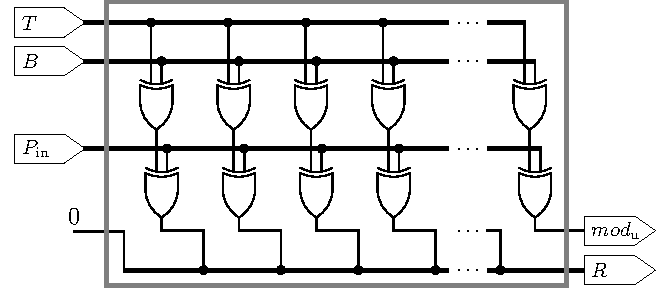
\includegraphics[width=12cm]{malu-basic}
		\caption{MALU - Basis ontwerp met shift\label{figuur-implementatie-malu-basic}}
\end{figure}

Aangezien voor het ontwerp het veld en de modulo veelterm op voorhand bepaald zijn, is het mogelijk een zeer groot aantal XOR poorten uit het ontwerp te verwijderen. De ingang $P$ en de bijhorende $m$ XOR poorten kunnen vervangen worden door een 1 bit `modulo enable' ingang $mod_{\text{e}}$ en er worden enkel XOR poorten geplaatst voor de bits $i$ waarvoor $P_i = 1$. Hierdoor wordt het aantal ingangen drastisch verkleind en worden 
\[\Delta = m - (\textsf{Hamm}(P) - 1)\]
XOR poorten uitgespaard.

In dit geval is $m = 163$ en $P = z^{163} + z^7 + z^6 + z^3 + 1$. Er zijn dus $\textsf{Hamm}(P) - 1 = 4$ XOR poorten nodig, wat een besparing van $163 - 4 =  159$ XOR poorten oplevert ($51\%$ minder dan het oorsponkelijk aantal).

De resulterende schakeling is te zien in \reffig{figuur-implementatie-malu-optimized}.

\begin{figure}[h]
	\centering
		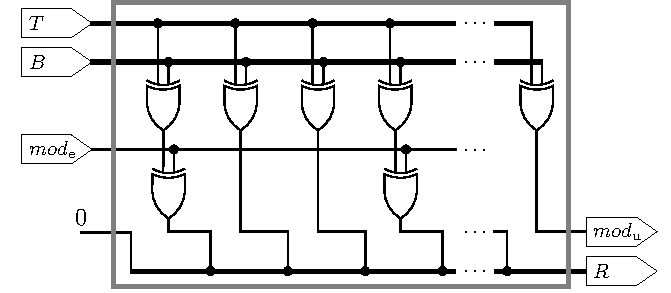
\includegraphics[width=12cm]{malu-optimized}
		\caption{MALU - Geoptimaliseerd ontwerp met shift\label{figuur-implementatie-malu-optimized}}
\end{figure}

\section{$\mathbb{F}_{2^m}$\label{sectie-implementatie-gf2m} kern}

\subsection{Basisontwerp\label{subsectie-implementatie-gf2m-basisontwerp}}

De eerder ontworpen MALU schakeling laat toe optellingen te doen, maar het Miller algoritme vereist dat er ook vermenigvuldigingen worden uitgerekend. Delingen en machtsverheffingen kunnen met behulp van vermenigvuldiging berekend worden en dienen dus niet rechtstreeks ge\"implementeerd te worden. Indien dus zowel optellingen als vermenigvuldigingen berekend kunnen worden, is alles voorhanden om de Tate pairing te berekenen.

Door toepassing van een ``shift and add'' algoritme, kan de waarde van \mbox{$A \cdot B = R$} berekend worden met behulp van de MALU schakeling. In \refalg{algoritme-implementatie-gf2m-multiply} is te zien hoe dit juist in z'n werk gaat. Door de modulo bewerking telkens op het tussenresultaat uit te voeren, is het steeds van graad $\leq m$ en kan het opgeslagen worden in $T$. Op het einde moet het resultaat door $z$ gedeeld worden, wat neerkomt op een verschuiving van alle bits met 1 plaats naar rechts.

\begin{algorithm}[h]
	\caption{``Shift and add'' vermenigvuldiging in $\mathbb{F}_{2^m}$}
	\label{algoritme-implementatie-gf2m-multiply}
	\KwIn{$A, B \in \mathbb{F}_{2^m}$}
	\KwOut{$R = A \cdot B \in \mathbb{F}_{2^m}$}
	\KwData{$T \in \mathbb{F}_{2^{m + 1}}$}
	\SetKwFunction{Degree}{degree}

	$T \gets 0$\;
	\For{$i \gets m - 1$ \KwTo $0$}{
		\eIf{$A_i = 1$}{
			$b \gets B$\;
		}{
			$b \gets 0$\;
		}
	
		$T \gets T \xor b$\;
	
		\If{$\Degree{T} = m$}{
			$T \gets T \xor P$\;
		}
		$T \gets T \ll 1$\;
	}
	$R \gets T \gg 1$\;
\end{algorithm}

Wanneer de optelling en vermenigvuldiging nu in een schakeling gegoten worden, dient te schakeling te weten welke van de twee bewerkingen moet uitgevoerd worden. Verder moet het mogelijk zijn de uitkomt $R$ in het register $T$ op te slaan. Op die manier is het mogelijk de uitgang van de schakeling gelijk te stellen aan $R$ zolang geen nieuwe berekening gestart wordt.  

Verderop zal gezien worden dat in het Miller algoritme verscheidene keren de som $R + 1$ moet berekend worden. Daarom wordt aan de schakeling een ingang $plus\_one$ toegevoegd die hierin helpt voorzien. De uiteindelijke schakeling is te zien in \reffig{figuur-implementatie-wrapper-gf2m}. Er wordt zo veel mogelijk bespaard op registers. Het register $cycle$ (equivalent aan $i$ in \refalg{algoritme-implementatie-gf2m-multiply}) is $\lceil \log _2 (m) \rceil$ bits lang en register $T$ $m$ bits. De waarde van $T_m$ wordt opgeslagen in register $mod$. Alle overige registers zijn 1 bit groot. Merk dus op dat de variabele $T$ uit \refalg{algoritme-implementatie-gf2m-multiply} hier gevormd wordt door de combinatie van de registers $T$ en $mod$. 

Voor $A$ wordt geen appart register voorzien en in plaats van $A_i$ wordt steeds bit $A_m$ ingelezen voor de vermenigvuldiging. De schakeling die van deze schakeling gebruik maakt, dient dus te voorzien in een methode om elke klokslag de juiste $A_i$ aan te bieden op $A_m$. Dit kan simpelweg gebeuren door elke klokslag na de start van de berekening het register dat $A$ bevat \'e\'en positie naar links door te schuiven.

\begin{figure}[h]
	\centering
		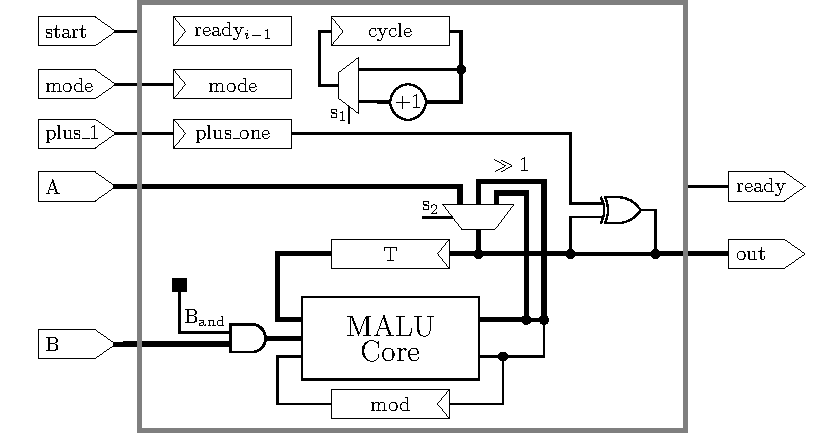
\includegraphics[width=12cm]{wrapper-gf2m}
		\caption{Schakeling voor $\mathbb{F}_{2^m}$ kern\label{figuur-implementatie-wrapper-gf2m}}
\end{figure}

Gezien de eenvoud van de schakeling is het niet nodig een FSM te implementeren, de besturing kan volledig via logica gebeuren. Die wordt getoond in \reffig{figuur-implementatie-wrapper-gf2m-logica}. De werking is zeer eenvoudig: zo lang $start$ hoog is, worden de registers $mode$ en $plus\_one$ geladen met hun respectievelijke ingangen. Verder wordt, afhankelijk van $mode$, $F$ ingeladen met de waarde van $A$ (optelling, $mode = 0$) of gelijkgesteld aan nul (vermenigvuldiging, $mode = 1$). Ook wordt $cycle$ gereset. Wanneer $start$ laag is, wordt, afhankelijk van de gewenste bewerking en de waarde van $ready$, het register $T$ geladen met de uitgang $R$ van de MALU of het uiteindelijke resultaat $R_{\text{ready}} = R \gg 1$.

\begin{figure}[h]
	\centering
		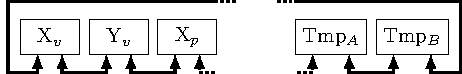
\includegraphics[width=12cm]{wrapper-gf2m-logica}
		\caption{Logica voor besturing van de $\mathbb{F}_{2^m}$ kern\label{figuur-implementatie-wrapper-gf2m-logica}}
\end{figure}

\subsection{Versnelling van de vermenigvuldiging\label{subsectie-implementatie-gf2m-versnelling}}

Wanneer met behulp van de schakeling in \reffig{figuur-implementatie-wrapper-gf2m} een vermenigvuldiging wordt berekend, zal het $m$ klokcycli duren eer het resultaat beschikbaar is aan de uitgang. Het is echter mogelijk dat aantal drastisch naar beneden te halen door $d$ MALU's te gebruiken en dus $d$ optellingen per klokcyclus uit te voeren. Het principe hiervan wordt ge\"illustreerd in \reffig{figuur-implementatie-wrapper-gf2m-d}.

\begin{figure}[h]
	\centering
		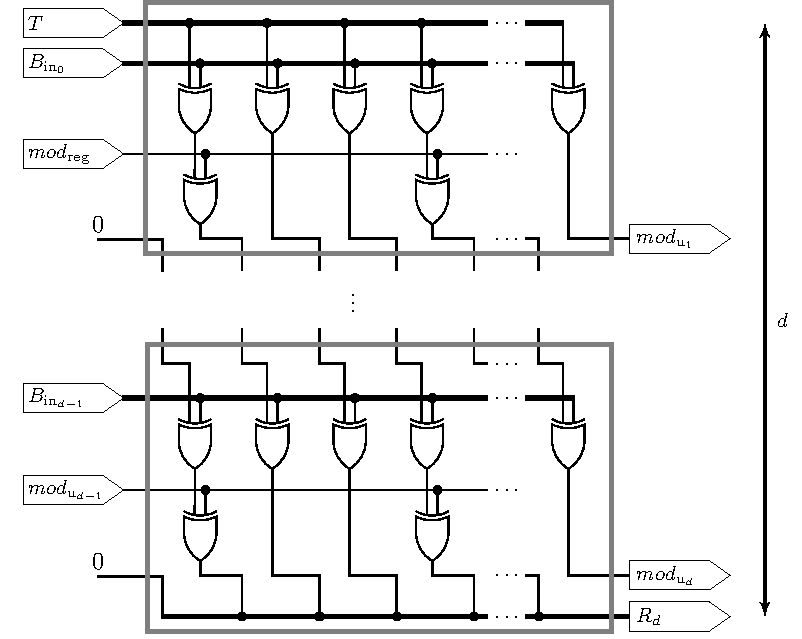
\includegraphics[width=12cm]{malu-width-d}
		\caption{Aaneenschakeling van $d$ MALU's ter versnelling van de vermenigvuldiging\label{figuur-implementatie-wrapper-gf2m-d}}
\end{figure}

De rekentijd van het Miller algoritme zal door toepassing van deze techniek gevoelig verkort kunnen worden. Hoe groter $m$ en hoe meer vermenigvuldigigen er uitgevoerd dienen te worden, des te significanter de tijdswinst die geboekt kan worden. Uiteraard gaat het gebruik van deze techniek wel in tegen de eerder opgelegde beperking aan de grootte van de uiteindelijke schakeling. Het is echter niet zo dat er enkel $d - 1$ extra MALU blokken dienen toegevoegd te worden, afhankelijk van $d$ en $m$ dient ook een extra multiplexer in de schakeling gestoken te worden. Dit is zoals opgemerkt in \refsect{sectie-implementatie-beperkingen} een zeer slechte zaak voor de  oppervlakte.

Stel bijvoorbeeld $d = 4$ (en $m = 	163$). Het resultaat van een optelling zal net zoals in het standaard ontwerp (\reffig{figuur-implementatie-wrapper-gf2m}) aanwezig zijn aan de uitgang van MALU \nr 1. Het resultaat van een vermenigvuldiging zal echter aan de uitgang van MALU \nr 3 verschijnen, aangezien $163 \bmod 4 = 3$. Het eindresultaat dat in register $T$ dient opgeslagen te worden, is voor een vermenigvuldiging dus
\[R_{3_{\text{ready}}} = mod{\text{u}_3} \text{ \# } R_{3_{162:1}},\]
terwijl dit voor een optelling
\[R_{1_{\text{ready}}} = mod_{\text{u}_1} \text{ \# } R_{1_{162:1}}\]
is. Met andere woorden, er dient nu niet enkel gekozen te kunnen worden tussen de ingangen $A$, $R_d$ of $R_{1_{\text{ready}}}$, maar ook voor $R_{3_{\text{ready}}}$.

Indien men toch wenst het vermenigvuldigen te versnellen, is het aangeraden een $d$ te kiezen waarvoor $m \bmod d = 1$. Als voorbeeld worden enkele voor de hand liggende en optimale keuzes vergeleken voor $d$ indien $m = 163$ in \reftbl{tabel-implementatie-woordbreedte-d}.

\begin{table}[h]
	\caption{Locatie van het resultaat van een vermenigvuldiging voor $d$ MALU's indien \mbox{$m=163$}}
	\label{tabel-implementatie-woordbreedte-d}

	\centering
	\begin{tabular}{lcccccc}
		\toprule
		\multicolumn{7}{c}{Voor de hand liggende waarden voor $d$}\\
		\midrule
		$d$			& 2	& 4	& 8	& 16	& 32	& 64\\
		$m \bmod d \qquad$	& 1	& 3	& 3	& 3	& 3	& 35\\
		\bottomrule
		\multicolumn{7}{c}{}\\
		\toprule
		\multicolumn{7}{c}{Optimale waarden voor $d$}\\
		\midrule
		$d$			& 2	& 3	& 6	& 9	& 18	& 27\\
		$m \bmod d$	& 1	& 1	& 1	& 1	& 1	& 1\\
		\bottomrule
	\end{tabular}
\end{table}

\section{Controller voor het Miller algoritme\label{sectie-implementatie-miller}}

\subsection{Algemeen ontwerp\label{subsectie-implementatie-miller-ontwerp}}

Nu een schakeling voorhanden is die toelaat alle benodigde berekeningen uit te voeren, rest nog een schakeling te ontwerpen die het Miller algoritme (zie \refsect{sectie-pairings-berekening}) uitvoert. Het algoritme met invulling van de vastgelegde parameters, zonder uitwerking van de berekeningen, wordt gegeven in \refalg{algoritme-implementatie-miller-algemeen}.

\begin{algorithm}[h]
	\caption{Miller algoritme voor de Tate pairing met parameters ingevuld}
	\label{algoritme-implementatie-miller-algemeen}
	\KwIn{$P, Q \in E(\mathbb{F}_{2^{163}})$}
	\KwOut{$e(P, Q)$}
	$F \gets 1$\;
	$V \gets P$\;
	\For{$i \gets 162$ \KwTo $0$}{
		$F \gets F^2 \cdot G_{V,V}(\phi(Q))$\;\nllabel{lijn-implementatie-miller-algemeen-double-1}
		$V \gets 2 \cdot V$\;\nllabel{lijn-implementatie-miller-algemeen-double-2}
		\If{$i = 82$}{\nllabel{lijn-implementatie-miller-algemeen-add-if}
			$F \gets F \cdot G_{V,P}(\phi(Q))$\;\nllabel{lijn-implementatie-miller-algemeen-add-1}
			$V \gets V + P$\;\nllabel{lijn-implementatie-miller-algemeen-add-2}
		}
	}
	$e(P, Q) \gets F^{\frac{2^{4 \cdot 163} - 1}{2^{163} + 2^{82} + 1}}$\;
	\KwRet{$e(P, Q)$}
\end{algorithm}

Merk op dat op lijn~\ref{lijn-implementatie-miller-algemeen-add-if} slechts \'e\'en waarde moet nagekeken worden, aangezien $l = 2^{163} + 2^{82} + 1$.

De controller zal ontworpen worden zoals het schema in \reffig{figuur-implementatie-miller-controller}. Voor het geheugenblok volledig ontworpen kan worden, moeten echter eerst de verschillende berekeningen uitgewerkt worden. Vervolgens zal aan de hand van die uitwerkingen bepaald worden hoeveel registers ten minste noodzakelijk zijn. Afhankelijk van diezelfde uitwerkingen zullen ook enkele geheugen elementen voor tellers en statusbits toegevoegd moeten worden. Ten slotte zal een FSM ontworpen worden.

\begin{figure}[h]
	\centering
		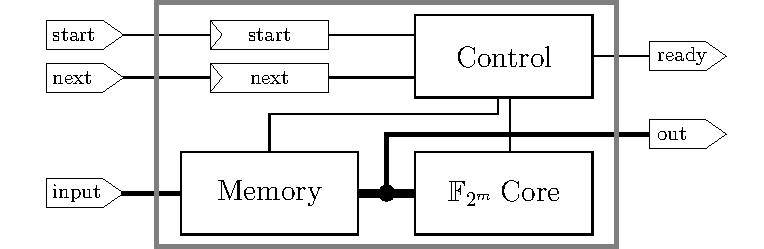
\includegraphics[width=12cm]{controller-miller}
		\caption{Schakeling voor de uitvoering van het Miller algoritme\label{figuur-implementatie-miller-controller}}
\end{figure}

Grofweg kan het algoritme opgedeeld worden in de for-lus  en een finale machtsverheffing. De for-lus kan verder onderverdeeld worden in een verdubbelstap, een optelstap, een kwadratering van F en een vermenigvuldiging $F \cdot G$. Elk van deze stappen zal verder uitgediept worden en er zal voor elke berekening bepaald worden hoeveel tussenresultaten minimum opgeslagen moeten worden. Het zal blijken dat een inversie in $\mathbb{F}_{2^m}$ uitgerekend moet kunnen worden, wat ook verder uitgediept zal worden.

Bij elk van de volgende algoritmen zal aangegeven worden hoeveel en welke bewerkingen juist nodig zijn. Daarbij staat \textsf{A} voor een optelling, \textsf{M} voor een vermenigvuldiging, \textsf{S} voor een kwadratering en \textsf{I} voor een inversie. Aangezien er echter geen afzonderlijke schakeling voor kwadrateren ontworpen is, zijn \textsf{S} en \textsf{M} qua rekentijd in dit geval equivalent aan elkaar. De bewerking $a + 1$ neemt geen extra tijd in beslag, omdat die functie parallel met een optelling of vermenigvuldiging kan uitgevoerd worden door de $plus\_one$ van de $\mathbb{F}_{2^m}$ kern hoog te maken bij de start van een berekening.

\subsection{For-lus\label{subsectie-implementatie-miller-forlus}}

Zoals reeds eerder vermeld kan de for-lus onderverdeeld worden in een verdubbelstap, een optelstap, een kwadratering van F en een vermenigvuldiging $F \cdot G$. Elk van deze onderdelen zal in de volgende paragrafen in detail aan bod komen.

\subsubsection{Verdubbelstap}

De verdubbelstap wordt gevormd door lijnen \ref{lijn-implementatie-miller-algemeen-double-1} en \ref{lijn-implementatie-miller-algemeen-double-2} in \refalg{algoritme-implementatie-miller-algemeen}. Voor een supersinguliere kromme zijn de berekeningen als volgt \cite{bertoni, hankerson-book}:

\[\begin{aligned}
	\lambda &= x_V^2 + 1\\
	x_{2V} &= \lambda ^2\\
	y_{2V} &= \lambda \cdot (x_{2V} + x_V) + y_V + 1\\
	G_{V,V}(\phi(Q)) &= \lambda \cdot (x_{\phi} + x_V) + (y_{\phi} + y_V)\\
\end{aligned}\]

In dit geval kan $y_{2V}$ ook berekend worden als:
\[\begin{aligned}
y_{2V}	&= y_V^4 + x_V^4\\
			&= (y_V + x_V)^4\\
\end{aligned}\]
Aangezien dit echter twee kwadrateringen en een optelling kost tegenover een vermenigvuldiging en twee optellingen, wordt de voorkeur gegeven aan de eerste methode.

Door de specifieke vorm van $\phi(Q)$ kan $G$ uitgeschreven worden als:

\[\begin{aligned}
	G_a	&=	\lambda \cdot (x_{\phi_a} + x_V) + (y_{\phi_a} + y_V)\qquad&
				G_c	&= \lambda \cdot x_{\phi_c} + y_{\phi_c}\\
	G_b	&=	\lambda \cdot x_{\phi_b} + y_{\phi_b}&
						&= 0\\
			&= \lambda + y_{\phi_b}&
				G_d	&= \lambda \cdot x_{\phi_d} + y_{\phi_d}\\
			&=	\lambda + x_{\phi_a}&
						&= 1\\
\end{aligned}\]

De variabele $G$ kan dus opgeslagen worden in twee registers van grootte $m$ in plaats van in vier. De vorm van $G$ zal ook toelaten de vermenigvuldiging $F \cdot G$ grotendeels te vereenvoudigen, zoals later gezien zal worden.

Tanneer dit in rekening gebracht wordt en het algoritme op register niveau wordt uitgeschreven, bekomt men uiteindelijk \refalg{algoritme-implementatie-miller-double-detail}. Hierbij werd specifiek gelet op een minimum gebruik van tijdelijke registers.

Buiten zes registers voor $x_{2V}$, $y_{2V}$, $x_{\phi_a}$, $y_{\phi_a}$, $G_a$ en $G_b$, is er ook \'e\'en register nodig om $\lambda$ in op te slaan. In totaal moeten er zes optellingen, twee vermenigvuldigingen en twee kwadrateringen uitgerekend worden.

\begin{algorithm}[h]
	\caption{Uitwerking van de verdubbelstap voor supersinguliere krommen in het Miller algoritme}
	\label{algoritme-implementatie-miller-double-detail}
	\KwIn{$x_V, y_V \in E(\mathbb{F}_{2^m})$; $x_{\phi_a}, y_{\phi_a} \in \mathbb{F}_{2^m}$}
	\KwOut{$x_{2V}, y_{2V} \in E(\mathbb{F}_{2^m})$; $G \in \mathbb{F}_{2^{4m}}$}
	\KwData{$\lambda \in \mathbb{F}_{2^m}$}
	$G_a \gets x_V$; $G_b \gets y_V$\;
	$\lambda \gets G_a^2 + 1$; $x_{2V} \gets \lambda ^2$\comm{2 S}\;
	$y_{2V} \gets x_{2V} + G_a$; $y_{2V} \gets y_{2V} \cdot \lambda$\comm{1 M, 1 A}\;
	$y_{2V} \gets y_{2V} + G_b + 1$\comm{1 A}\;
	$G_a \gets G_a + x_{\phi_a}$; $G_a \gets G_a \cdot \lambda$\comm{1 M, 1 A}\;
	$G_a \gets G_a + y_{\phi_a}$; $G_a \gets G_a + G_b$\comm{2 A}\;
	$G_b \gets \lambda + x_{\phi_a}$\comm{1 A}\;
\end{algorithm}

\subsubsection{Optelstap}

De optelstap bestaat uit lijnen \ref{lijn-implementatie-miller-algemeen-add-1} en \ref{lijn-implementatie-miller-algemeen-add-2} van \refalg{algoritme-implementatie-miller-algemeen}. Voor een supersinguliere kromme dienen de volgende bewerkingen uitgevoerd te worden \cite{bertoni, hankerson-book}:

\[\begin{aligned}
	\lambda &= \frac{y_V + y_P}{x_V + x_P}\\
	x_{V + P} &= \lambda ^2 + x_V + x_P\\
	y_{V + P} &= \lambda \cdot (x_{V + P} + x_P) + y_P + 1\\
	G_{V,P}(\phi(Q)) &= \lambda \cdot (x_{\phi} + x_P) + (y_{\phi} + y_P)\\
\end{aligned}\]

Net zoals bij de verdubbelstap kan $G$ hier in twee variabelen opgeslagen worden. Hoewel de optelstap slechts \'e\'en maal moet worden uitgevoerd, is het uiteraard cruciaal dat ook hier zo weinig mogelijk tijdelijke variabelen gebruikt worden. Op die manier blijft de grootte van de uiteindelijke schakeling het kleinst. De uitgewerkte versie van het algoritme wordt gegeven in \refalg{algoritme-implementatie-miller-add-detail}.

In tegenstelling tot de verdubbelstap zijn hier twee tijdelijke registers nodig, een voor $\lambda$ en een voor $a$. Verder zijn er twee registers nodig voor $x_P$ en $y_P$. Alles samen dienen er tien optellingen, drie vermenigvuldigingen, twee kwadrateringen en een inversie uitgerekend te worden.

\begin{algorithm}[h]
	\caption{Uitwerking van de optelstap voor supersinguliere krommen in het Miller algoritme}
	\label{algoritme-implementatie-miller-add-detail}
	\KwIn{$x_V, y_V, x_P, y_P \in E(\mathbb{F}_{2^m})$; $x_{\phi_a}, y_{\phi_a} \in \mathbb{F}_{2^m}$}
	\KwOut{$x_{V + P}, y_{V + P} \in E(\mathbb{F}_{2^m})$; $G \in \mathbb{F}_{2^{4m}}$}
	\KwData{$\lambda, a \in \mathbb{F}_{2^m}$}
	$G_a \gets x_V$; $G_b \gets y_V$\;
	$\lambda \gets G_a + x_P$; $\lambda \gets \lambda^{-1}$\comm{1 I, 1 A}\;
	$a \gets G_b + y_P$; $\lambda \gets \lambda \cdot a$\comm{1 M, 1 A}\;
	$x_{V + P} \gets \lambda ^2 + G_a$; $x_{V + P} \gets x_{V + P} + x_P$\comm{1 S, 2 A}\;
	$y_{V + P} \gets x_{V + P} + x_P$; $y_{V + P} \gets y_{V + P} \cdot \lambda$\comm{1 M, 1 A}\;
	$y_{V + P} \gets y_{V + P} + y_P + 1$\comm{1 A}\;
	$G_a \gets x_{\phi_a} + x_P$; $G_a \gets G_a \cdot \lambda$\comm{1 M, 1 A}\;
	$G_a \gets G_a + y_{\phi_a}$; $G_a \gets G_a + y_P$\comm{2 A}\;
	$G_b \gets \lambda + x_{\phi_a}$\comm{1 A}\;
\end{algorithm}

\subsubsection{Inversie}

De meest tijdrovende stap in de optelstap is de inversie.  Een inversie in een Galois veld kan berekend worden door toepassing van de kleine stelling van Fermat:

\[\begin{aligned}
a^{2^m}		&= a\\
a^{2^m - 1}	&= 1\\
a^{2^m - 2}	&= a^{-1}\\
\end{aligned}\]

% $2^{163} -2 = 11 692 013 098 647 223 345 629 478 661 730 264 157 247 460 343 806$

De na\"ieve manier om dit te berekenen zou zijn om $a$ in totaal $2^m - 2$ maal met zichzelf te vermenigvuldigingen. In dit geval zou dat betekenen dat er $2^{163} - 2$ vermenigvuldigingen moeten uitgevoerd worden, wat uiteraard onhaalbaar is.

Een tweede manier bestaat er in de exponent te ontbinden in machten van 2 en 3. In dat geval zouden er nog 237 vermenigvuldigen nodig zijn.

Er is echter een derde, optimale manier die toegepast kan worden indien de exponent van de vorm $2^m - 2$ is \cite{batina-pkc, itoh}. Dit gaat als volgt in zijn werk. Stel:
\[a^{2^m - 2} = (a^{2^{m - 1} - 1})^2\]
Als wordt aangenomen dat $m$ oneven is, is de exponent van twee na het gelijkheidsteken dus even. Zolang de exponent even is, kan recursief volgende formule toegepast worden:
\[a^{2^i - 1} = (a^{2^{\frac{i}{2}} - 1})^{2^{\frac{i}{2}}} \cdot a^{2^{\frac{i}{2}} - 1}\]
Indien $a$ oneven is, dient volgende formule toegepast te worden:
\[a^{2^i - 1} = (a^{2^{i - 1} - 1})^2 \cdot a\]
Uiteindelijk eindigt men dan bij $a^2$. Het totaal aantal bewerkingen voor een inversie in $\mathbb{F}_{2^m}$ is $\lfloor\log_2(m - 1)\rfloor + \textsf{Hamm}(m - 1) + 1$ vermenigvuldigingen en $m - 1$ kwadrateringen.

In het geval van $m = 163$ is de uiteindelijke keten van bewerkingen zoals gegeven in \refalg{algoritme-implementatie-miller-inversie}. Het aantal berekeningen in dat geval is 9 vermenigvuldigingen en 162 kwadrateringen. Er is een register nodig om $a$ bij de houden en twee voor de tussenresultaten $a^{2^i - 1}$ en $(a^{2^i - 1})^{2^i}$.

\begin{algorithm}[h]
	\caption{Inversie in $\mathbb{F}_{2^{163}}$}
	\label{algoritme-implementatie-miller-inversie}
	\KwIn{$a \in \mathbb{F}_{2^{163}}$}
	\KwOut{$a^{-1} \in \mathbb{F}_{2^{163}}$}
	$a^3 \gets a^2 \cdot a$\comm{1 S, 1 M}\;
	$a^{2^4 - 1} \gets (a^3)^{2^2} \cdot a^3$\comm{2 S, 1 M}\;
	$a^{2^5 - 1} \gets (a^{2^4 - 1})^2 \cdot a$\comm{1 S, 1 M}\;
	$a^{2^{10} - 1} \gets (a^{2^5 - 1})^{2^5} \cdot a^{2^5 - 1}$\comm{5 S, 1 M}\;
	$a^{2^{20} - 1} \gets (a^{2^{10} - 1})^{2^{10}} \cdot a^{2^{10} - 1}$\comm{10 S, 1 M}\;
	$a^{2^{40} - 1} \gets (a^{2^{20} - 1})^{2^{20}} \cdot a^{2^{20} - 1}$\comm{20 S, 1 M}\;
	$a^{2^{80} - 1} \gets (a^{2^{40} - 1})^{2^{40}} \cdot a^{2^{40} - 1}$\comm{40 S, 1 M}\;
	$a^{2^{81} - 1} \gets (a^{2^{80} - 1})^2 \cdot a$\comm{1 S, 1 M}\;
	$a^{2^{162} - 1} \gets (a^{2^{81} - 1})^{2^{81}} \cdot a^{2^{81} - 1}$\comm{81 S, 1 M}\;
	$a^{-1} \gets (a^{2^{162} - 1})^2$\comm{1 S}\;
\end{algorithm}

\subsubsection{Kwadratering van $F$}

Bij het uitvoeren van lijn~\ref{lijn-implementatie-miller-algemeen-double-1} van \refalg{algoritme-implementatie-miller-algemeen} moet ook telkens het kwadraat van $F$ berekend worden. De afleiding van de formule daarvoor gaat als volgt:

\[\begin{aligned}
F^2	&= (F_a + F_b x + F_c y + F_d xy) \cdot (F_a + F_b x + F_c y + F_d xy)\\
		&= F_a^2 + F_a F_b x + F_a F_c y + F_a F_d xy + F_b F_a x + F_b^2 x^2 + F_b F_c xy\\
			&\quad + F_b F_d x^2y + F_c F_a y + F_c F_b xy + F_c^2 y^2 + F_c F_d xy^2 + F_d F_a xy\\
			&\quad + F_d F_b x^2y + F_d F_c xy^2 + F_d^2 x^2 y^2\\
		&= (F_a^2 + F_b^2 + F_c^2 + F_d^2)\\
			&\quad + (F_a F_b + F_b F_a + F_b^2 + F_c F_d + F_d F_c + F_d^2)x\\
			&\quad + (F_a F_c + F_b F_d + F_c F_a + F_c^2 + F_c F_d + F_d F_b + F_d F_c)y\\
			&\quad + (F_a F_d + F_b F_c + F_b F_d + F_c F_b + F_c^2 + F_d F_a + F_d F_b + F_d^2)xy\\
		&= (F_a^2 + F_b^2 + F_c^2 + F_d^2) + (F_b^2 + F_d^2)x + F_c^2 y + (F_c^2 + F_d^2)xy\\
\end{aligned}\]

Mist de originele waarde van $F$ overschreven mag worden, is het mogelijk dit te berekenen zonder gebruik van tijdelijke variabelen. Er zijn dus enkel vier registers nodig voor $F$. Hoe dat in z'n werk gaat is te zien in \refalg{algoritme-implementatie-miller-f-square}. E\'en kwadratering van $F$ vraagt vier optellingen en vier kwadrateringen in $\mathbb{F}_{2^m}$.

\begin{algorithm}[h]
	\caption{Uitwerking van van $F^2 \in \mathbb{F}_{2^{4m}}$}
	\label{algoritme-implementatie-miller-f-square}
	\KwIn{$F = F_a + F_b x + F_c y + F_d xy \in \mathbb{F}_{2^{4m}}$}
	\KwOut{$F = F^2 \in \mathbb{F}_{2^{4m}}$}
	$F_a \gets F_a + F_c$\comm{1 A}\;
	$F_a \gets F_a^2$\comm{1 S}\;
	$F_b \gets F_b + F_d$\comm{1 A}\;
	$F_b \gets F_b^2$\comm{1 S}\;
	$F_a \gets F_a + F_b$\comm{1 A}\;
	$F_c \gets F_c^2$\comm{1 S}\;
	$F_d \gets F_d^2$\comm{1 S}\;
	$F_d \gets F_d + F_c$\comm{1 A}\;
\end{algorithm}

\subsubsection{Vermenigvuldiging $F \cdot G$}

Zoals eerder opgemerkt, is $G$ in zowel de verdubbel- als optelstap niet van volledige rang in het extensieveld. De vermenigvuldiging van F met G kan daardoor vereenvoudigd worden, namelijk als volgt:

\[\begin{aligned}
F \cdot G	&= (F_a + F_b x + F_c y + F_d xy) \cdot (G_a + G_b x + xy)\\
	&= F_a G_a + F_a G_b x + F_a xy + F_b G_a x + F_b G_b x^2 + F_b x^2y + F_c G_a y\\
		&\quad + F_c G_b xy + F_c xy^2 + F_d G_a xy + F_d G_b x^2y + F_d x^2 y^2\\
	&= (F_a G_a + F_b G_b + F_d)\\
		&\quad + (F_a G_b + F_b G_a + F_b G_b + F_c + F_d)x\\
		&\quad + (F_b + F_c G_a + F_c + F_d G_b)y\\
		&\quad + (F_a + F_b + F_c G_b + F_d G_a + F_d G_b + F_d)xy\\
\end{aligned}\]

Indien hier nu de Karatsuba-Ofman techniek \cite{karatsuba-oldest, zuras} op wordt toegepast, bekomt men:

\[\begin{aligned}
F \cdot G &= (F_a G_a + F_b G_b + F_d)\\
				&\quad + ((F_a + F_b) \cdot (G_a + G_b) + F_a G_a + F_c + F_d)x\\
				&\quad + (F_c G_a + F_d G_b + F_b + F_c)y\\
				&\quad + ((F_c + F_d) \cdot (G_a + G_b) + F_c G_a + F_a + F_b + F_d)xy\\
\end{aligned}\]

Deze formule kan uitgerekend wordt met gebruik van drie tijdelijke registers ($a$, $b$ en $c$). Verder zijn er vier registers nodig voor $F$ en twee voor $G$. Merk op dat de oude waarde van $F$ overschreven wordt door het resultaat. In totaal zijn er zes vermenigvuldigingen en veertien optellingen nodig. \refalg{algoritme-implementatie-miller-fg} beschrijft welke berekeningen juist uitgevoerd moeten worden.

Mist het gebruik van een vierde tijdelijk register zou het mogelijk zijn de berekening $G_a + G_b$ op te slaan. Die wordt nu zowel in lijn~\ref{lijn-implementatie-miller-fg-gagb-1} als \ref{lijn-implementatie-miller-fg-gagb-2} berekend. Er zouden dan slechts dertien optellingen moeten berekend worden, \'e\'en minder dan \cite{beuchat}, waar $y^2 + y +x$ gebruikt wordt als modulo veelterm voor het extensieveld. Aangezien een extra tijdelijk register echter tegen de doelstellingen ingaat, wordt voor de iets langere berekening gekozen.

\begin{algorithm}[h]
	\caption{Uitwerking van de vermenigvuldiging $F \cdot G$ in het Miller algoritme}
	\label{algoritme-implementatie-miller-fg}
	\KwIn{$F = F_a + F_b x + F_c y + F_d xy, G = G_a + G_b x + xy \in \mathbb{F}_{2^{4m}}$}
	\KwOut{$F = F \cdot G \in \mathbb{F}_{2^{4m}}$}
	\KwData{$a, b, c \in \mathbb{F}_{2^m}$}
	$a \gets F_a \cdot G_a$; $a \gets a + F_d$\comm{1 M, 1 A}\;
	$b \gets F_a + F_b$; $c \gets G_a + G_b$\comm{2 A}\;\nllabel{lijn-implementatie-miller-fg-gagb-1}
	$b \gets b \cdot c$; $b \gets b + a$; $b \gets b + F_c$\comm{1 M, 2 A}\;
	$c \gets F_b \cdot G_b$; $a \gets a + c$\comm{1 M, 1 A}\;
	$c \gets F_c \cdot G_a$;	$c \gets c + F_b$\comm{1 M, 1 A}\;
	$F_b \gets b$; $b \gets c$\;
	$c \gets F_c + F_d$; $G_a \gets G_a + G_b$\comm{2 A}\;\nllabel{lijn-implementatie-miller-fg-gagb-2}
	$c \gets c \cdot G_a$; $c \gets c + b$; $c \gets c + F_a$\comm{1 M, 2 A}\;
	$F_a \gets a$\;
	$c \gets c + F_d$; $b \gets b + F_c$; $a \gets F_d \cdot G_b$\comm{1 M, 2 A}\;
	$F_c \gets b + a$; $F_d \gets c$\comm{1 A}\;
\end{algorithm}

\subsection{Finale machtsverheffing\label{subsectie-implementatie-miller-finale-exp}}

Eens de for-loop voltooid is, moet $F$ nog gereduceerd worden zodat het eindresultaat $e(P, Q)$ uniek is. Hoe dit gebeurt, wordt onderzocht in de volgende paragrafen. De gebruikte methodes zijn gebaseerd op die in \cite{beuchat}, aangepast aan het gekozen extensieveld en geoptimaliseerd om het registerverbruik zo laag mogelijk te houden.

De reductie op het einde van het Miller algoritme bestaat uit de machtsverheffing $e(P, Q) = F^M$, met
\[\begin{aligned}
M	&= \frac{2^{4m} - 1}{l}\\
	&= \frac{(2^{2m} + 1)(2^{2m} - 1)}{l}\\
	&= (2^{2m} - 1)(2^m - \nu 2^{\frac{m + 1}{2}} + 1)\\
	&= (2^{2m} - 1)(2^m + 1) + \nu(1 - 2^{2m})2^{\frac{m + 1}{2}}\\
\end{aligned}\]

Aangezien $\nu = 1$ in dit geval, kan de machtsverheffing dus berekend worden als
\[e(P, Q) = \left(F^{2^{2m} - 1}\right)^{2^m + 1} \cdot \left(F^{1 - 2^{2m}}\right)^{2^{\frac{m + 1}{2}}}\]

Er zal onderzocht worden hoe elk van deze termen berekend kan worden. Stel
\[\begin{aligned}
F	&= (F_a + F_b x) + (F_c + F_d x)y\\
	&= U_0 + U_1y,\\
\end{aligned}\]
met $U_0, U_1 \in \mathbb{F}_{2^{2m}}$. Met $y^{2^{2m}} = y + x + 1$ is $F^{2^{2m}} = U_0 + U_1 + U_1x + U_1y$. 	Men vindt dus:
\[\begin{aligned}
I  &= F^{2^{2m} - 1} = \frac{F^{2^{2m}}}{F}\\
	&= \frac{U_0 + U_1 + U_1x + U_1y}{U_0 + U_1y}\\
	&= \frac{(U_0 + U_1 + U_1x + U_1y)^2}{(U_0 + U_1 + U_1x + U_1y) \cdot (U_0 + U_1y)}\\
%	&= \frac{U_0^2 + U_1^2 + U_1^2x + U_1^2y + U_1^2xy}{U_0^2 + U_1^2 + U_0 U_1 + U_0 U_1 x}\\
	&= \frac{U_0^2 + U_1^2 + U_1^2x}{U_0^2 + U_1^2 + U_0 U_1 + U_0 U_1 x} + \left[\frac{U_1^2 + U_1^2x}{U_0^2 + U_1^2 + U_0 U_1 + U_0 U_1 x}\right]y\\
\end{aligned}\]
en
\[\begin{aligned}
J  &= F^{1 - 2^{2m}} = \frac{F}{F^{2^{2m}}}\\
	&= \frac{U_0 + U_1y}{U_0 + U_1 + U_1x + U_1y}\\
	&= \frac{(U_0 + U_1y)^2}{(U_0 + U_1 + U_1x + U_1y) \cdot (U_0 + U_1y)}\\
%	&= \frac{U_0^2 + U_1^2 + + U_1^2y + U_1^2xy}{U_0^2 + U_1^2 + U_0 U_1 + U_0 U_1 x}\\
	&= \frac{U_0^2 + U_1^2}{U_0^2 + U_1^2 + U_0 U_1 + U_0 U_1 x} + \left[\frac{U_1^2 + U_1^2x}{U_0^2 + U_1^2 + U_0 U_1 + U_0 U_1 x}\right]y\\
\end{aligned}\]

Er moeten dus vier termen in $\mathbb{F}_{2^{2m}}$ berekend worden. Merk echter op dat de noemers van alle breuken in zowel $I$ als $J$ identiek zijn. Er zal dus slechts \'e\'en inversie in $\mathbb{F}_{2^{2m}}$ uitgerekend moeten worden. Ook zijn de tweede termen van $I$ en $J$ identiek. In totaal moeten dus drie elementen in $\mathbb{F}_{2^{2m}}$ opgeslagen worden alvorens de termen  vermenigvuldigd kunnen worden. Dit wil zeggen dat er dus zes registers van grootte $m$ nodig zijn.

\subsubsection{Termen van de deelbreuken}

Ten eerste worden de drie tellers $I_t$, $J_t$ en $G_t$ uitgewerkt. Hierbij staan $I_t$ en $J_t$ voor de teller van de eerste breuk van respectievelijk $I$ en $J$, $G_t$ staat voor de teller van de gemeenschappelijke tweede breuk en $G_n$ voor de gemeenschappelijke noemer. Met andere woorden:

\[\begin{aligned}
I = \frac{I_t}{G_n} + \left[ \frac{G_t}{G_n} \right] y\\
J = \frac{J_t}{G_n} + \left[ \frac{G_t}{G_n} \right] y\\
\end{aligned}\]

Het kwadraat van een element $A \in \mathbb{F}_{2^{2m}}$ is
\[\begin{aligned}
A^2	&= a_0^2 + a_1^2 x^2\\
		&= (a_0^2 + a_1^2) + a_1^2 x\\
\end{aligned}\]
en de vermenigvuldiging van $A, B \in \mathbb{F}_{2^{2m}}$:
\[\begin{aligned}
A \cdot B	&= a_0 b_0 + a_0 b_1 x + a_1 b_0 x + a_1 b_1 x^2\\
				&= (a_0 b_0 + a_1 b_1) + (a_0 b_1 + a_1 b_0 + a_1 b_1)x\\
\end{aligned}\]

Zodoende bekomt men:
\[\begin{aligned}
I_t	&= [(F_a^2 + F_b^2) + F_b^2 x] + [(F_c^2 + F_d^2) + F_d^2x] + [F_d^2 + F_c^2x]\\
		&= (F_a^2 + F_b^2 + F_c^2) + (F_b^2 + F_c^2 + F_d^2)x\\
J_t	&= [(F_a^2 + F_b^2) + F_b^2 x] + [(F_c^2 + F_d^2) + F_d^2x]\\
		&= (F_a^2 + F_b^2 + F_c^2 + F_d^2) + (F_b^2 + F_d^2)x\\
G_t	&= [(F_c^2 + F_d^2) + F_d^2x] + [F_d^2 + F_c^2x]\\
		&= F_c^2 + (F_c^2 + F_d^2)x\\
\end{aligned}\]

Voor de gemeenschappelijke noemer $G_n$ vind men:

\[\begin{aligned}
G_n	&= [(F_a^2 + F_b^2) + F_b^2 x] + [(F_c^2 + F_d^2) + F_d^2x]\\
			&\quad + [(F_a F_c + F_b F_d) + (F_a F_d + F_b F_c + F_b F_d)x]\\
			&\quad + [F_a F_d + F_b F_c + F_b F_d) + (F_a F_c + F_a F_d + F_b F_c)x]\\
		&= (F_a^2 + F_b^2 + F_c^2 + F_d^2 + F_a F_c + F_a F_d + F_b F_c)\\
			&\quad + (F_b^2 + F_d^2 + F_a F_c + F_b F_d)x\\
		&= (F_a^2 + F_b^2 + F_c^2 + F_d^2 + (F_a + F_b) \cdot (F_c + F_d) + F_b F_d)\\
			&\quad + (F_b^2 + F_d^2 + F_a F_c + F_b F_d)x\\
\end{aligned}\]

Een methode om deze vier resultaten uit te rekenen is te zien in \refalg{algoritme-implementatie-miller-final-noemers}. Er zijn vier registers nodig voor $F$ en acht voor $I_t$, $J_t$, $G_t$ en $G_n$. Tevens moet er nog \'e\'en tijdelijk register voorzien worden voor $a$. De uitkomsten kunnen bepaald worden na twaalf optellingen, drie vermenigvuldigingen en vier kwadrateringen.

\begin{algorithm}[h]
	\caption{Uitwerking van berekening van noemers voor de finale machtsverheffing in het Miller algoritme}
	\label{algoritme-implementatie-miller-final-noemers}
	\KwIn{$F = F_a + F_b x + F_c y + F_d xy \in \mathbb{F}_{2^{4m}}$}
	\KwOut{$I_t = I_{t_a} + I_{t_b} x, J_t = J_{t_a} + J_{t_b} x, G_t = G_{t_a} + G_{t_b} x$, \mbox{$G_n = G_{n_a} + G_{n_b} x$} $\in \mathbb{F}_{2^{2m}}$}
	\KwData{$a \in \mathbb{F}_{2^m}$}
	$I_{t_a} \gets F_a^2$; $I_{t_b} \gets F_b^2$; $G_{t_a} \gets F_c^2$; $G_{t_b} \gets F_d^2$\comm{4 S}\;
	$I_{t_a} \gets I_{t_a} + I_{t_b}$; $J_{t_b} \gets I_{t_b} + G_{t_b}$\comm{2 A}\;
	$G_{t_b} \gets I_{t_b} + G_{t_b}$; $J_{t_a} \gets I_{t_a} + G_{t_b}$\comm{2 A}\;
	$I_{t_a} \gets I_{t_a} + G_{t_a}$; $I_{t_b} \gets I_{t_b} + G_{t_b}$\comm{2 A}\;
	$G_{n_a} \gets F_a + F_b$; $G_{n_b} \gets J_a \cdot J_c$\comm{1 M, 1 A}\;
	$a \gets F_c + F_d$; $G_{n_a} \gets G_{n_a} \cdot a$; $a \gets F_b \cdot F_d$\comm{2 M, 1 A}\;
	$G_{n_a} \gets G_{n_a} + a$; $G_{n_b} \gets G_{n_b} + a$\comm{2 A}\;
	$G_{n_a} \gets G_{n_a} + J_{t_a}$; $G_{n_b} \gets G_{n_b} + J_{t_b}$\comm{2 A}\;
\end{algorithm}

\subsubsection{Inversie in $\mathbb{F}_{2^{2m}}$}

Vervolgens moet de inverse van $G_n$ berekend worden, wat een inversie in $\mathbb{F}_{2^{2m}}$ is \cite{beuchat}.

Stel $A = A_a + A_b x \in \mathbb{F}_{2^{2m}}, A \neq 0$ met multiplicatieve inverse $B = B_a + B_b x \in \mathbb{F}_{2^{2m}}$. Volgens de definitie is $A \cdot B = 1$. Gegeven $x^2 = x + 1$, gelden dus de vergelijkingen:

\[\left\{\begin{array}{l}
A_a B_a + A_b B_b = 1\\
A_a B_b + A_b B_a + B_b A_a = 0\\
\end{array}\right.\]

De oplossing van dit stelsel is

\[\begin{aligned}
B_a	&= w^{-1} \cdot (A_a + A_b),\\
B_b	&= w^{-1} \cdot A_b\\
\end{aligned}\]

met $w = A_a^2 + (A_a + A_b) \cdot A_b$. Een inversie in $\mathbb{F}_{2^{2m}}$ kan dus berekend worden via een inversie in $\mathbb{F}_{2^m}$. Uitgewerkt geeft dit \refalg{algoritme-implementatie-miller-f2m-inverse}, waarbij de oorspronkelijke $A$ wordt overschreven door zijn inverse. Het algoritme kost in totaal drie vermenigvuldigingen, \'e\'en kwadratering, twee optellingen en \'e\'en inversie in $\mathbb{F}_{2^m}$. Er zijn twee registers nodig om $A$ in op te slaan en drie tijdelijke registers voor $a$, $b$ en $c$. Verder heeft het algoritme voor inversie in $\mathbb{F}_{2^m}$ twee tijdelijke registers nodig, waarbij tijdelijk register $b$ de taak van \'e\'en van deze twee kan vervullen, aangezien dat niet meer gebruikt wordt na regel~\ref{lijn-implementatie-miller-f2m-inverse-b} in het algoritme. Dit alles samen komt dus neer op vier tijdelijke registers.

\begin{algorithm}[h]
	\caption{Uitwerking van $A^{-1} \in \mathbb{F}_{2^{2m}}$}
	\label{algoritme-implementatie-miller-f2m-inverse}
	\KwIn{$A = A_a + A_b x \in \mathbb{F}_{2^{2m}}, A \neq 0$}
	\KwOut{$B = A^{-1} = B_a + B_b x \in \mathbb{F}_{2^{2m}}$}
	\KwData{$a, b, c \in \mathbb{F}_{2^m}$}
	$a \gets A_a + A_b$; $b \gets A_a^2$\comm{1 S, 1 A}\;
	$c \gets a \cdot A_b$; $c \gets c + b$\comm{1 M, 1 A}\nllabel{lijn-implementatie-miller-f2m-inverse-b}\;
	$c \gets c^{-1}$\comm{1 S}\;
	$B_a \gets a \cdot c$; $B_b \gets A_b \cdot c$\comm{2 M}\;
\end{algorithm}

\subsubsection{Berekening van $I$ en $J$}

Gewapend met al deze waarden is het mogelijk $I = I_0 + I_1 y$ en $J = J_0 + J_1 y$ te berekenen. In totaal zijn hier zes vermenigvuldigingen in $\mathbb{F}_{2^{2m}}$ nodig. 

Stel $A = A_a + A_b x, B = B_a + B_b x \in \mathbb{F}_{2^{2m}}$. De vermenigvuldiging kan dan geschreven worden als:

\[\begin{aligned}
C	&= (A_a + A_b x) + (B_a + B_b x)\\
	&= (A_a B_a + A_b B_b) + (A_a B_b + A_b B_a + A_b B_b)x\\
	&= (A_a B_a + A_b B_b) + \bigl( (A_a + A_b) \cdot (B_a + B_b) + A_a B_a \bigr) x\\
\end{aligned}\]

In dit geval dienen zowel $I_t$, $J_t$ als $G_t$ met $G_n^{-1}$ vermenigvuldigd te worden. Vooropgesteld dat de tellers na vermenigvuldiging met $G_n$ niet meer nodig zijn en dus overschreven mogen worden, kan \refalg{algoritme-implementatie-miller-f2m-mult} gebruikt worden. Er zijn dan zes registers nodig voor de uitkomsten, twee voor $G_n^{-1}$ en twee tijdelijke register voor $a$ en $b$. De vermenigvuldiging in $\mathbb{F}_{2^{2m}}$ kan berekend worden in drie vermenigvuldigingen en vier optellingen.

\begin{algorithm}[h]
	\caption{Uitwerking van $A \cdot B \in \mathbb{F}_{2^{2m}}$}
	\label{algoritme-implementatie-miller-f2m-mult}
	\KwIn{$A = A_a + A_b x, B = B_a + B_b x \in \mathbb{F}_{2^{2m}}$}
	\KwOut{$A = A \cdot B \in \mathbb{F}_{2^{2m}}$}
	\KwData{$a, b \in \mathbb{F}_{2^m}$}
	$a \gets A_b \cdot B_b$; $b \gets A_a + A_b$\comm{1 M, 1 A}\;
	$A_a \gets A_a \cdot B_a$; $A_b \gets B_a + B_b$\comm{1 M, 1 A}\;
	$A_b \gets A_b \cdot b$\comm{1 M}\;
	$A_b \gets A_a + A_b$; $A_a \gets A_a + a$\comm{2 A}\;
\end{algorithm}

\subsubsection{Berekening van $I^{2^m + 1}$}

Nu $I$ en $J$ bekend zijn, moeten ze beiden tot de correcte macht verheven worden. Voor $I$ is dat $2^m + 1$, wat simpelweg mogelijk zou zijn door $I^{2^m}$ te berekenen en dit resultaat te vermenigvuldigen met $I$. Dit zou een vermenigvuldiging van twee elementen in $\mathbb{F}_{2^{4m}}$ zijn, wat, zoals verderop zal gezien worden, negen vermenigvuldigingen en twee\"entwintig optellingen kost. Er is echter een snellere manier.

Uitgaande van de gelijkheid $A^{2^m} = A$ voor $A \in \mathbb{F}_{2^{m}}$, weet men dat de vier elementen van $I$ na de machtsverheffing simpelweg zullen bestaan uit sommen van de beginwaarden. Via volgende gelijkheden:

\[\begin{aligned}
x^{2^m}	&= 1 + x\\
y^{2^m}	&= 1 + x + y + xy\\
(xy)^{2^m}	&= x + xy\\
\end{aligned}\]
en met $I = I_a + I_b x + I_c y + I_d xy$, vindt men dus:
\[I^{2^m} = (I_a + I_b + I_c) + (I_b + I_c + I_d) x + I_c y + (I_c + I_d) xy.\]
Vervolgens vermenigvuldigt men dit met de originele $I$, wat resulteert in $I^{2^m + 1} = r_a + r_b x + r_c y + r_d xy$:
\[\begin{aligned}
r_a	&= (I_a + I_b + I_c) \cdot I_a + (I_b + I_c + I_d) \cdot I_b + I_c^2 + (I_c + I_d) \cdot I_d\\
r_b	&= (I_a + I_b + I_c) \cdot I_b + (I_b + I_c + I_d) \cdot I_a + (I_b + I_c + I_d) \cdot I_b\\
		&\quad + I_c I_d + (I_c + I_d) \cdot I_c + (I_c + I_d) \cdot I_d\\
r_c	&= (I_a + I_b + I_c) \cdot I_c + (I_b + I_c + I_d) \cdot I-d + I_a I_c + I_c^2 + I_c I_d\\
		&\quad + (I_c + I_d) \cdot I_b + (I_c + I_d) \cdot I_c\\
r_d	&= (I_a + I_b + I_c) \cdot I_d + (I_b + I_c + I_d) \cdot I_c + (I_b + I_c + I_d) \cdot I_d\\
		&\quad + I_b I_c + I_c^2 + (I_c + I_d) \cdot I_a + (I_c + I_d) \cdot I_b + (I_c + I_d) \cdot I_d.\\
\end{aligned}\]
Dit kan vereenvoudigd worden tot:
\[\begin{aligned}
r_a	&= I_a^2 + I_a I_b + I_a I_c + I_b^2 + I_b I_c + I_b I_d + I_c^2 + I_c I_d + I_d^2\\
r_b	&= I_a I_c + I_a I_d + I_b I_d + I_c I_d + I_c^2 + I_d^2\\
r_c	&= I_c^2 + I_c I_d + I_d^2\\
r_d	&= I_a I_c + I_b I_c + I_b I_d.\\
\end{aligned}\]

Voor de toepassing van de Karatsuba-Ofman techniek worden de volgende tussenresultaten uitgerekend:
\[\begin{aligned}
m_0	&= (I_a + I_b) \cdot (I_c + I_d)
			&\quad m_1	&= I_a I_b\\
m_2	&= I_a I_d
			&m_3	&= I_b I_c\\
m_4	&= I_c I_d\\
s_0	&= (I_a + I_b)^2
			&s_1	&= (I_c + I_d)^2.\\
\end{aligned}\]
Aan de hand van deze waarden kan het uiteindelijke resultaat berekend worden:
\[\begin{aligned}
I^{2^m + 1}	&= (m_0 + m_1 + m_2 + m_4 + s_0 + s_1)\\
				&\quad + (m_0 + m_3 + m_4 + s_1) x \\
				&\quad + (m_4 + s_1) y + (m_0 + m_2) xy.\\
\end{aligned}\]

Ook bij de implementatie van dit algoritme wordt er van uit gegaan dat de beginvariable, $I$ in dit geval, niet behouden dient te worden. Er zijn dan uiteindelijk vier registers nodig voor het resultaat en vijf voor tussenresultaten. De totale kost komt neer op vijf vermenigvuldigingen, twee kwadrateringen en negen optellingen. \refalg{algoritme-implementatie-miller-v-power} geeft een overzicht van de bewerkingen.

\begin{algorithm}[h]
	\caption{Uitwerking van $I^{2^m + 1} \in \mathbb{F}_{2^{4m}}$}
	\label{algoritme-implementatie-miller-v-power}
	\KwIn{$I = I_a + I_b x + I_c y + I_d xy \in \mathbb{F}_{2^{4m}}$}
	\KwOut{$I = I^{2^m + 1} \in \mathbb{F}_{2^{4m}}$}
	\KwData{$a, b, \ldots, e \in \mathbb{F}_{2^m}$}
	$a \gets I_a \cdot I_b$; $b \gets I_a + I_b$\comm{1 M, 1 A}\;
	$c \gets b^2$; $d \gets I_a \cdot I_d$\comm{1 M, 1 S}\;
	$I_b \gets I_b \cdot I_c$; $e \gets I_c + I_d$\comm{1 M, 1 A}\;
	$b \gets b \cdot e$; $e \gets e^2$\comm{1 M, 1 S}\;
	$I_c \gets I_c \cdot I_d$\comm{1 M}\; 
	$I_c \gets I_c + e$; $I_a \gets I_c + b$\comm{2 A}\;
	$I_b \gets I_a + I_b$; $I_d \gets b + d$\comm{2 A}\;
	$b \gets c + d$; $I_a \gets I_a + b$\comm{2 A}\;
	$I_a \gets I_a + a$\comm{1 A}\;
\end{algorithm}

\subsubsection{Berekening van $J^{2^{\frac{m + 1}{2}}}$}

De voorlaatste berekening die gemaakt moet worden, is de machtsverheffing van $J$. Helaas is het in dit geval niet mogelijk om de bewerking even snel uit te voeren als de kwadratering van $I$. De handigste oplossing in dit geval is $J$ simpelweg $\frac{m + 1}{2}$ opeenvolgende keren te kwadrateren. Hiervoor kan \refalg{algoritme-implementatie-miller-f-square} gebruikt worden. In totaal zal deze stap $2 \cdot (m + 1)$ vermenigvuldigigen en optellingen vragen, wat voor de gekozen $m = 163$ neerkomt op 328 maal beide bewerkingen.

\subsubsection{Vermenigvuldiging van $I \cdot J$}

De finale stap is de vermenigvuldiging van de twee resulterende variabelen $I$ en $J$. Dit is een vermenigvuldiging in $\mathbb{F}_{2^{4m}}$ en deze kan als volgt geformuleerd worden:

\[\begin{aligned}
e(P, Q)	&= I \cdot J\\
	&= (I_a J_a + I_b J_b + I_c J_c + I_d J_d)\\
	&\quad + (I_a J_b + I_b J_a + I_b J_b + I_c J_d + I_d J_c + I_d J_d)x\\
	&\quad + (I_a J_c + I_b J_d + I_c J_a + I_c J_c + I_d J_d + I_d J_b + I_d J_c)y\\
	&\quad + (I_a J_d + I_b J_c + I_b J_d + I_c J_b + I_c J_c + I_d J_a + I_d J_b + I_d J_d)xy\\
\end{aligned}\]

Om de berekening via de Karatsuba-Ofman techniek te versnellen, worden eerst volgende tussenresultaten uitgerekend:

\[\begin{aligned}
m_0	&= I_a J_a
	&m_1	&= I_b J_b\\
m_3	&= I_c J_c
	&m_4	&= I_d J_d\\
l_0	&= (I_a + I_b) \cdot (J_a + J_b)
	&\quad l_1	&= (I_c + I_d) \cdot (J_c + J_d)\\
l_2	&= (I_a + I_d) \cdot (J_a + J_d)
	&l_3	&= (I_a + I_c) \cdot (J_a + J_c)\\
n_0	&= I_a + I_b + I_c + I_d
	&n_1	&= J_a + J_b + J_c + J_d\\
p_0	&= n_0 \cdot n_1\\
\end{aligned}\]

Gebruik makende van deze waarden, kan de vermenigvuldiging voor $e(P, Q)$ geschreven worden als:
\[\begin{aligned}
e(P, Q)	&= (m_0 + m_1 + m_2 + m_3) + (m_0 + m_2 + l_0 + l_1)x\\
	&\quad + (m_0 + m_1 + m_2 + l_1 + l_2 + l_3)y\\
	&\quad + (m_0 + m_3 + l_0 + l_1 + l_3 + p_0)xy\\
\end{aligned}\]

Indien zowel $I$ als $J$ overschreven mogen worden, is de minimum benodigde opslagruimte om deze berekeningen uit te voeren vier registers voor het eindresultaat $I = e(P, Q)$ en zes tijdelijke registers voor $a, b, \ldots, f$. Dit alles samen vergt negen vermenigvuldigingen en twee\"entwintig optellingen, twee meer dan in \cite{beuchat}. De methode is terug te vinden in \refalg{algoritme-implementatie-miller-f4m-mult}.

\begin{algorithm}
	\caption{Uitwerking van $I \cdot J \in \mathbb{F}_{2^{4m}}$}
	\label{algoritme-implementatie-miller-f4m-mult}
	\KwIn{$I = I_a + I_b x + I_c y + I_d xy, J = J_a + J_b x + J_c y + J_d xy \in \mathbb{F}_{2^{4m}}$}
	\KwOut{$I = I \cdot J \in \mathbb{F}_{2^{4m}}$}
	\KwData{$a, b, \ldots, f \in \mathbb{F}_{2^m}$}
	$a \gets J_c + J_d$; $b \gets J_b + J_d$\comm{2 A}\;
	$J_d \gets I_d \cdot J_d$; $c \gets I_b + I_d$\comm{1 M, 1 A}\;
	$I_d \gets I_c + I_d$; $d \gets I_b \cdot J_b$\comm{1 M, 1 A}\;
	$e \gets I_a + I_b$; $f \gets J_a + J_b$\comm{2 A}\;
	$I_b \gets J_a + J_c$; $J_c \gets I_c \cdot J_c$\comm{1 M, 1 A}\;
	$J_a \gets I_a \cdot J_a$; $I_a \gets I_a + I_c$\comm{1 M, 1 A}\;
	$I_c \gets I_a \cdot I_b$; $J_b \gets c \cdot b$\comm{2 M}\;
	$I_a \gets e \cdot f$; $I_b \gets I_d \cdot a$ \comm{2 M}\;
	$I_d \gets e + I_d$; $e \gets J_a + I_b$\comm{2 A}\;
	$I_b \gets f + a$; $I_d \gets I_b \cdot I_d$\comm{1 M, 1 A}\;
	$a \gets e + I_a$; $I_b \gets J_c + a$\comm{2 A}\;
	$I_a \gets d + J_c$; $I_d \gets I_d + J_d$\comm{2 A}\;
	$I_d \gets I_d + a$; $I_d \gets I_c + I_d$\comm{2 A}\;
	$I_c \gets I_c + e$; $I_c \gets I_c + J_b$\comm{2 A}\;
	$I_c \gets I_c + I_a$; $I_a \gets J_d + I_a$\comm{2 A}\;
	$I_a \gets I_a + J_a$\comm{1 A}\;
\end{algorithm}

\subsection{Geheugen}

Nu alle nodige algoritmes en de daarbij horende geheugenvereisten gekend zijn, is het mogelijk om het geheugenblok van de schakeling te ontwerpen. Eerst zal het minimum aantal benodigde registers bepaald worden en vervolgens zal een ontwerp voor het geheugenblok voorgesteld worden.

\subsubsection{Minimum aantal registers}

De geheugenvereisten van de for-lus en de finale machtsverheffing kunnen los van elkaar bekeken worden. Eens de lus be\"eindigd is, is het immers niet meer nodig $P, \phi(Q), V$ en $G$ bij te houden.

Van de vijf algoritmes die opgeroepen worden in de for-lus, vereist de de vermenigvuldiging van $F$ en $G$ het grootste aantal tijdelijke registers, namelijk drie. Het minimum aantal registers om alle bewerkingen in de lus te kunnen uitvoeren is dus vijftien: zes voor $P, \phi(Q)$ en $V$, twee voor $G$, vier voor $F$ en drie tijdelijke registers.

Bij de berekening van de finale machtsverheffing gaat de vermenigvuldiging van $I$ en $J$ met de titel van `meest geheugenvereisende' algoritme lopen. In dit geval zijn er veertien registers nodig: acht voor $I$ en $J$ en zes voor de tussenresultaten.

Het minimum aantal registers $n$ is dus vijftien. In totaal bevat de complete schakeling zestien registers van grootte $m$: vijftien in de controller voor het Miller algoritme en \'e\'en in de $\mathbb{F}_{2^m}$ kern.

\subsubsection{Ontwerp van het geheugenblok}

Voor het ontwerp van het geheugenblok wordt RAM al op voorhand verworpen gezien dit zowel groot is als veel vermogen verbruikt. Er wordt verder gebouwd op de idee\"en aangebracht in \cite{lee}. Daarin wordt een circulair ontwerp voorgesteld dat ge\"illustreerd wordt in \reffig{figuur-implementatie-miller-geheugen-circ}. Het voordeel van zo'n ontwerp ten opzichte van RAM is de veel kleinere oppervlakte. Bij RAM stijgt de complexiteit van de oppervlakte van de multiplexers kwadratisch met het aantal registers. Bij een ontwerp van dit type is de complexiteit van de multiplexers echter constant met als resultaat een veel kleinere implementatie.

\begin{figure}[h]
	\centering
		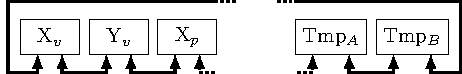
\includegraphics[width=12cm]{geheugen-circ}
		\caption{Circulair registerblokontwerp en mogelijke bewerkingen\label{figuur-implementatie-miller-geheugen-circ}}
\end{figure}

Elk van de registers kan enkel de waarde van zijn voorganger aannemen (de zogenaamde \emph{shift} bewerking). Tevens kunnen de waarden van eerste twee registers omgewisseld worden (\emph{swap}) en kan de waarde van register twee naar register \'e\'en gekopieerd worden (\emph{copy}). De ingangen van de wiskundige schakeling (de $\mathbb{F}_{2^m}$ kern in dit geval) zijn rechtstreeks verbonden met registers \'e\'en en twee. Aan register \'e\'en zijn tevens ook de uitgang van de wiskundige schakeling en de ingang van de volledige schakeling aangesloten. De enige manier om nieuwe waarden in de registers op te slaan, is dus via de aanpassing van de waarde van register \'e\'en. %Tevens worden ingangen $A$ en $B$ voor de $\mathbb{F}_{2^m}$ kern vast verbonden met twee op voorhand bepaalde registers, alsook de uitgang $R$. 

Omdat de ingangen van de onderliggende $\mathbb{F}_{2^m}$ kern rechtstreeks verbonden zijn met twee registers, is het noodzakelijk om voor elke bewerking de nodige waarden naar die registers over te brengen. Het gemiddeld aantal klokcycli $\overline{t}$ dat daar voor nodig is, kan op de manier die volgt bepaald worden. Eerst wordt de gemiddelde afstand $\overline{r}$ tussen twee variabelen $x_0$ en $x_1$ bepaald. Die is gelijk aan de som $s$ van de mogelijke afstanden $r$ gedeeld door het aantal mogelijke posities $c$ die twee variabelen kunnen bezetten:
\[\begin{aligned}
s	&= \sum_{i = 1}^{n - 1} \sum_{j = i + 1}^n (j - i - 1)
	&\qquad c	&= \sum_{i = 0}^{n - 1} i\\
	&= \frac{n \cdot (n - 1) \cdot (n - 2)}{6}
	&	&= n \cdot \frac{n - 1}{2}\\
\end{aligned}\]
dus
\[\overline{r}	= \frac{n - 2}{3}.\]
Merk op dat deze formules slechts een benadering geven. Zo wordt bijvoorbeeld niet in rekening gebracht dat wanneer beide waarden in de eerste twee registers zitten, er geen doorschuivingen moeten gebeuren.

Per positie die $x_0$ en $x_1$ van elkaar verwijderd zijn, zal een \emph{swap} bewerking uitgevoerd moeten worden. Daartoe dient $x_1$ telkens eerst verplaatst te worden naar register twee. Er zijn dus $\overline{r} \cdot n$ doorschuif bewerkingen nodig. Dit is opnieuw een ruwe schatting, die voor kleine $n$ niet zal kloppen. Algemeen kan echter gesteld worden dat
\[\overline{t} \in O \Bigl( \frac{n^2}{3} \Bigr).\]

Verder is het energieverbruik recht evenredig met het aantal schrijfbewerkingen die op de registers worden uitgevoerd. Elke doorschuif bewerking kost $n$ zulke bewerkingen, m.a.w.\ het gemiddeld aantal schrijfbewerkingen $\overline{w}$ dat uitgevoerd moet worden voor gestart kan worden met de berekening van een optelling of vermenigvuldiging, is
\[\overline{w} \in O \Bigl( \frac{n^3}{3} \Bigr).\]

Gezien het feit dat er vijftien registers zijn (tegenover zes in \cite{lee}), zou dit zeer veel energie kosten. Verder zou het veel klokcycli in beslag nemen om beide waarden in de correcte registers op te slaan, hoewel zoals eerder bepaald tijdsduur niet van zeer groot belang is. Om dit probleem op te lossen, wordt het mogelijk gemaakt dat elk register ook de waarde van zijn voorganger kan opslaan. Dit is equivalent aan de \emph{swap} (en \emph{copy}) bewerking toelaten tussen alle aan elkaar grenzende registers. Verder kunnen \emph{swap} bewerkingen tussen twee paar registers in parallel uitgevoerd worden. Uiteraard wordt hiervoor een prijs betaald, er moet nu namelijk per register een extra multiplexer en een selectie signaal voorzien worden.  Het resulterend ontwerp is te zien in \reffig{figuur-implementatie-miller-geheugen-circ-optimized}.

\begin{figure}[h]
	\centering
		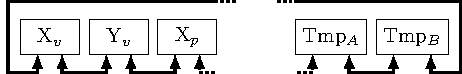
\includegraphics[width=12cm]{geheugen-circ-optimized}
		\caption{Circulair registerblok geoptimaliseerd voor laag energieverbruik\label{figuur-implementatie-miller-geheugen-circ-optimized}}
\end{figure}

In dit geval zal de afstand $r$ van een waarde $x$ tot het eerste register gelijk zijn aan $\textsf{min}(j - 1, n - j + 1)$ omdat nu in beide richtingen geschoven kan worden. De gemiddelde afstand $\overline{r}$ is dan
\[\begin{aligned}
\overline{r}	&= \frac{1}{n} \cdot \sum_{i = 1}^{n} \textsf{min}(j - 1, n - j + 1)\\
	&= \frac{2}{n} \cdot \sum_{i = 1}^{\frac{n}{2}} (j - 1)\\
	&= \frac{n - 1}{4}.
\end{aligned}\]
Aangezien de omwisselbewerkingen in parallel uitgevoerd kunnen worden, is het gemiddeld aantal klokcycli in dit geval
\[\overline{t} \in O  \Bigl( \frac{n}{4} \Bigr).\]
Rekening houdend met het feit dat elke omwisselbewerking twee schrijfbewerkingen vraagt en er twee variabelen naar de juiste positie gebracht moeten worden, geldt
\[\overline{w} \in O(n).\]

Tegenover het originele ontwerp voor het registerblok, zal dit ontwerp veel minder klokcycli verloren laten gaan aan het in de juiste positie brengen van de benodigde variabelen. Ook zal het, ten koste van meer multiplexers, minder energie verbruiken. De extra multiplexers zullen echter ook energie vragen, dus in hoeverre dit het totale energieverbruik naar beneden haalt, moet van implementatie tot implementatie bekeken worden. 

Registers \'e\'en en twee worden respectievelijk met de $A$ en $B$ ingang van de $\mathbb{F}_{2^m}$ kern verbonden. Om vermenigvuldigingen tot een succesvol einde te brengen, moet het register dat met de $A$ ingang verbonden is elke klokslag met $d$ bits naar links doorgeschoven kunnen worden. Hierbij gaat de originele waarde van het register echter wel verloren. Wanneer de algoritmes die het meeste tijdelijke opslag vragen echter nauwkeurig worden bekeken, zal men merken dat dit geen probleem vormt. Vandaar dat er voor gekozen wordt om het derde tijdelijk register uit de doorschuif lus te halen, er moeten dan minder doorschuivingen doorgevoerd worden om elke waarde in de juiste positie te brengen. Verder moet het ook mogelijk zijn waarden die op de ingang van de Miller controller aangelegd worden op te slaan en het resultaat op de uitgang te zetten. Ten slotte moet het resultaat van een berekening in $\mathbb{F}_{2^m}$ opgeslagen kunnen worden. Teneinde dat mogelijk te maken, wordt de uitgang $R$ van de $\mathbb{F}_{2^m}$ kern aan het derde tijdelijk register gekoppeld. Rekend houdend met deze zaken, wordt het ontwerp van de eerste twee registers aangepast zoals te zien in \reffig{figuur-implementatie-geheugen-eerste-twee}.

\begin{figure}[h]
	\centering
		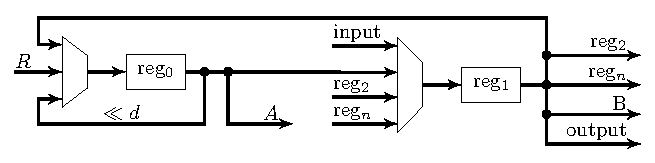
\includegraphics[width=12cm]{geheugen-eerste-twee}
		\caption{Ontwerp van de schakeling rond de eerste twee registers in het registerblok\label{figuur-implementatie-geheugen-eerste-twee}}
\end{figure}

\subsection{FSM}

Nut alle details over de hardware bekend zijn, kan overgegaan worden tot het ontwerp van een FSM. Daarbij zal een zeer groot deel van de te implementeren toestanden voor niets anders dienen dan het verschuiven van geheugen. Het uiteindelijke resultaat bevat 553 toestanden. Om het geheel overzichtelijk te houden, zal het ontwerp dan ook niet tot op individueel state niveau gebeuren. Ook zal zoveel mogelijk getracht worden reeds ge\"implementeerde toestanden opnieuw te gebruiken.

Aangezien een beeld meer zegt dan duizend woorden, wordt het resultaat zonder veel extra uitleg gepresenteerd in \reffig{figuur-miller-fsm}. De aanduidingen $start$ en $next$ staan voor de ingangen van de schakeling (zie \reffig{figuur-implementatie-miller-controller}). De aanduiding $\#next = 3$ wil zeggen: `aantal maal dat $next$ hoog werd is gelijk aan drie'. Een register $o$ geeft aan of de optelstap moet uitgevoerd worden en er is een teller $i$ die bijhoudt hoeveel stappen in de for-lus nog uitgevoerd moeten worden.

Wat wel enige extra aandacht verdient, is de opsplitsing van de verdubbel- en optelstap. Wanneer \refalg{algoritme-implementatie-miller-double-detail} en \ref{algoritme-implementatie-miller-add-detail} opnieuw bekeken worden, valt het op dat buiten de berekening van $\lambda$ en de nieuwe $x$-co\"ordinaat van $V$ alle andere berekeningen zeer gelijkaardig zijn. Meer nog, indien de paren $(x_V, y_V)$ en $(x_P, y_P)$ vervangen worden door een algemene $(x_A, y_A)$, dan bestaan beide algoritmes uit dezelfde bewerkingen na het berekenen van $\lambda$ en $x_V$. Aangezien na de berekening van $\lambda$ nog steeds twee registers vrij zijn voor gebruik, kunnen deze aangewend worden om de toepasselijke $x$ en $y$ co\"ordinaten in op te slaan. Op die manier kunnen de verdere berekeningen via dezelfde toestanden uitgewerkt worden, ongeacht of nu voordien de verdubbel- of de optelstap uitgevoerd werd.

\begin{figure}[h]
	\centering
		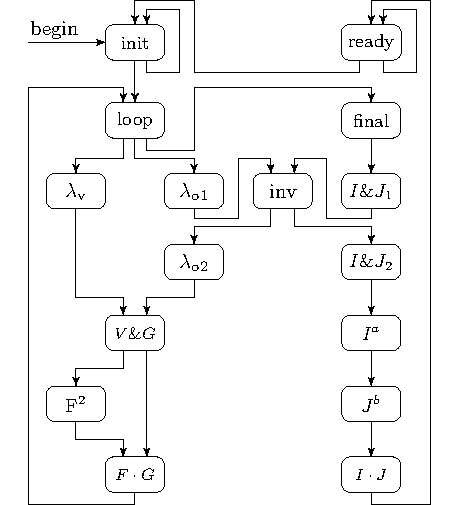
\includegraphics[scale=1]{miller-fsm}
		\caption{FSM ontwerp van de controller voor het Miller algoritme\label{figuur-miller-fsm}}
\end{figure}

\section{Optimalisaties\label{sectie-implementatie-optimalisaties}}

Nu de schakeling volledig ontworpen is, kan overgegaan worden tot optimalisering. Daarbij wordt opnieuw in de eerste plaats getracht de oppervlakte kleiner te maken, maar er zal ook aandacht gegeven worden aan het beperken van het energieverbruik van de schakeling. De optimalisaties die in de volgende paragrafen voorgesteld worden, zullen allemaal iets te maken hebben met de registers. Omdat de enkele registers van grootte $1$ of $\textsf{log}_2(m)$ bit (voor tellers) niet veel bijdragen aan de uiteindelijke oppervlakte of het energieverbruik, zullen de optimalisaties specifiek gericht zijn op het effici\"enter maken van het geheugenblok in de controller voor de Miller loop.

Een register is doorgaans opgebouwd uit een aantal D-type master-slave flip-flops. In de gebruikte bibliotheek \cite{cell-databook} is dit type flip-flops opgebouwd uit twee latches. De eerste latch (master) is verbonden met de ingang $D$ en laat de waarde daarvan door zolang $CLK$ laag is. De tweede latch (slave) is verbonden met de uitgang $Q$  en neemt de waarde van de eerste latch over eens $CLK$ hoog is. Het effect is dus dat de uitgang $Q$ op een stijgende klokflank de waarde van $D$ overneemt. Er bestaan verschillende gespecialiseerde types: met resetingang, met enable ingang, met test ingang, $\ldots$ In de paragrafen die volgen, wordt er van uit gegaan dat alle registers uit dit type flip-flops zijn opgebouwd.

\subsection{Registers zonder reset}

Een makkelijke eerste aanpassing is het verwijderen van de resetingangen van de registers. Zoals reeds gezien in \reftbl{tabel-implementatie-beperkingen-elementen-gatecount} kost een D flip-flop zonder resetingang 0,5 gate minder per bit dan \'e\'en met, een verkleining van $8,5\%$.

In het geval van $m = 163$ kijkt men dan aan tegen een besparing van $978 - 896,5 = 81,5$ gates per register. Merk echter wel op dat ten minste \'e\'en register moet overblijven dat wel op 0 (en 1) ingesteld kan worden om $F$ in te stellen aan het begin van het algoritme.

\subsection{Clock gating\label{subsectie-implementatie-optimalisatie-clock-gating}}

Normaal wordt een register elke klokslag geladen met de waarde aan zijn ingang. Het is dus noodzakelijk het register naar zichzelf terug te koppelen, zodat het mogelijk is een reeds opgeslagen waarde in het register te bewaren. Een techniek, genaamd clock gating, laat toe deze terugkoppeling (en de daarbij horende multiplexer) achterwege te laten \cite{low-power}. Bij deze techniek wordt het kloksignaal enkel gepropageerd naar een register wanneer een daarbij horende enable ingang hoog is. Zolang het enable signaal laag gehouden wordt, blijft de waarde van het register dus constant.

Deze techniek laat ook toe het verbruik van de schakeling drastisch te verlagen. Er zullen immers veel minder interne poorten zijn (bv. in de multiplexer) die elke klokslag van waarde dienen te veranderen.

De eenvoudigste schakeling waarmee clock gating ge\"implementeerd kan worden is te zien in \reffig{figuur-implementatie-optimalisatie-cg-basic}. Er zijn echter enkele problemen geassocieerd met dit type schakeling. De uitgang is immers onderhevig aan onregelmatigheden op het enable signaal. Stel bijvoorbeeld dat de enable ingang al hoog wordt terwijl het kloksignaal ook nog hoog is. Dan zal het kloksignaal gepropageerd worden tot het register, wat niet de bedoeling is.

\begin{figure}[h]
	\centering
		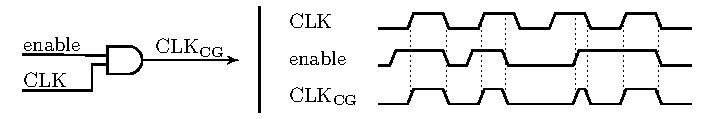
\includegraphics[scale=0.8]{cg-basic}
		\caption{Schakeling voor clock gating - Basis ontwerp\label{figuur-implementatie-optimalisatie-cg-basic}}
\end{figure}

Dit probleem kan verholpen worden met de schakeling voorgesteld in \reffig{figuur-implementatie-optimalisatie-cg-no-glitch}. De latch zorgt er hier voor dat het enable signaal pas wordt doorgelaten nadat het kloksignaal laag geweest is. Hierdoor worden mogelijke onregelmatigheden dus tegengehouden voor de ze klokingang van het register kunnen bereiken.

\begin{figure}[h]
	\centering
		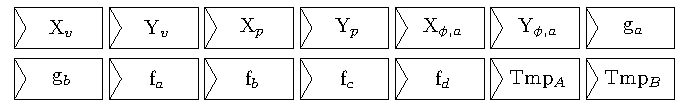
\includegraphics[scale=0.8]{cg-no-glitch}
		\caption{Schakeling voor clock gating - Verbeterd ontwerp\label{figuur-implementatie-optimalisatie-cg-no-glitch}}
\end{figure}

Ten slotte is er een derde oplossing die toelaat een nog grotere energiebesparing door te voeren, zoals aangetoond in \cite{mueller}. In die paper wordt bewezen dat het energie verbruik van een D-type master-slave flip-flop veel hoger is wanneer het kloksignaal laag is, dan wanneer het hoog is. De reden hiervan is duidelijk te zien in \reffig{figuur-implementatie-optimalisatie-cg-power-dis}: wanneer de klok laag is, veranderen, telkens de ingang verandert, twee interne poorten van staat en wijzigen de gate capaciteiten van twee andere poorten. Indien de klokingang hoog is, wijzigt een veranderend ingangssignaal enkel de gate capaciteit van de eerste interne poort.

\begin{figure}[h]
	\centering
		\subfigure[$CLK = 0$]{
			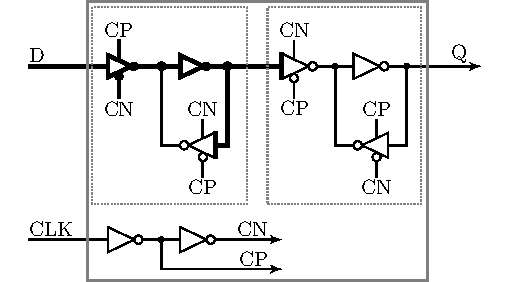
\includegraphics[width=5.7cm]{cg-pow-dis-zero}
			%\label{subfig-1-implementatie-optimalisatie-cg-power-dis}
		}
		\subfigure[$CLK = 1$]{
			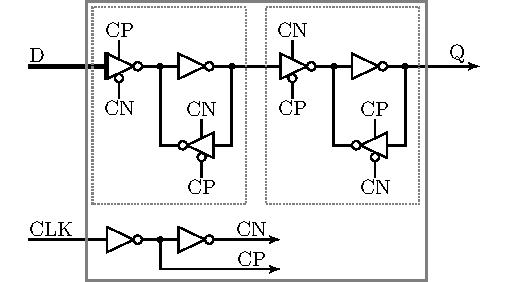
\includegraphics[width=5.7cm]{cg-pow-dis-one}
			%\label{subfig-2-implementatie-optimalisatie-cg-power-dis}
		}
		\caption[Vermogenverbruikende onderdelen van een D-type master-slave flip-flop bij constante waarde van de klok ingang]{Vermogenverbruikende onderdelen van een D-type master-slave flip-flop bij constante waarde van de klokingang \protect\cite{mueller}. De dikke lijnen geven de vermogenverbruikende onderdelen aan.\label{figuur-implementatie-optimalisatie-cg-power-dis}}
\end{figure}

De werking van de twee vorige schakelingen is zo dat de klokingang laag gehouden wordt zolang het enable signaal laag is. De oplossing ligt in de schakeling in \reffig{figuur-implementatie-optimalisatie-cg-low-power}, die exact doet wat nodig is: de klokingang hoog houden zolang geen nieuwe waarde moet opgeslagen worden. Om het voorkomen van onregelmatigheden te garanderen, moet het enable signaal stabiel worden voor het CLK signaal hoog wordt. Indien bepaalde kloksignaalbeperkingen worden opgelegd bij het synthetiseren van het circuit is dit normaal gezien echter geen probleem.

\begin{figure}[h]
	\centering
		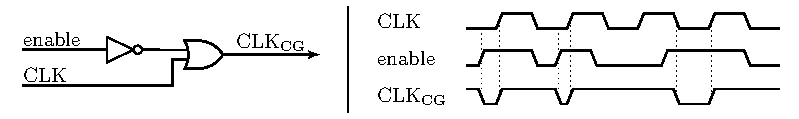
\includegraphics[scale=0.8]{cg-low-power}
		\caption{Schakeling voor clock gating - Laag vermogen ontwerp\label{figuur-implementatie-optimalisatie-cg-low-power}}
\end{figure}
		% Hardware implementatie
\Chapter{Resultaten\label{hfdst-resultaten}}

In dit hoofdstuk zal het ASIC ontwerp van de schakeling die in \refhfdst{hfdst-implementatie} beschreven werd van naderbij bestudeerd worden. Daarbij zal gekeken worden naar de oppervlakte van de schakeling, het verbruik en de maximum bereikbare kloksnelheid $f_{\text{max}}$. Er zal onderzocht worden wat het effect van de verschillende voorgestelde optimalisaties is op al deze parameters. Ten slotte zal het ontwerp vergeleken worden met reeds bestaande implementaties.

Het ontwerp werd geprogrammeerd in GEZEL \cite{gezel}. Simulaties en compilatie naar VHDL werden uitgevoerd met GEZEL 2.0. De optimalisaties werden doorgevoerd in de VHDL code, aangezien GEZEL dit niet toelaat. Alle ontwerpen werden gesynthetiseerd met behulp van Synopsys Design Vision. De gebruikte bibliotheek was de \emph{$0.13 \mu m$ low leakage} bibliotheek van Faraday Technology \cite{cell-databook}. Het werd de software verboden flip-flops met test ingangen te gebruiken. De maximale oppervlakte werd ingesteld op nul, wat als netto effect een resultaat met minimum oppervlakte gaf. Verder werd voor het kloksignaal een frequentie van 100kHz gedefini\"eerd.

De grootte van alle resultaten wordt uitgedrukt in gates. Dit laat toe te vergelijken met andere resultaten die in de literatuur terug te vinden zijn.

Voor de resultaten in verband met energieverbruik worden steeds twee waarden gegeven. De eerste waarde, dynamisch verbruik, geeft weer hoeveel vermogen verbruikt wordt door veranderende CMOS in- en uitgangen. De tweede waarde, leakage verbruik, is verbruik dat voorkomt zelfs indien een transistor niet geleidt. De impact hiervan hangt onder meer af van de gebruikte bibliotheek.

De beide waarden moeten met een stevige korrel zout genomen worden. Het is voor het synthese programma zeer moeilijk hier een nauwkeurige schatting voor te geven. Zolang twee schakelingen echter met dezelfde software, bibliotheek en parameters werden gesynthetiseerd, zijn relatieve vergelijkingen mogelijk. Stel bijvoorbeeld dat het verbruik van ontwerp A geschat wordt op $200 nW$ en dit van ontwerp B op $100 nW$. Indien er dan voldaan is aan de voorgenoemde voorwaarden, zal het effectief verbruik van B ongeveer de helft zijn van A. Het is dus in het algemeen niet aangeraden vergelijkingen omtrent verbruik te maken met andere bestaande ontwerpen aan de hand van de waarden gegeven in dit hoofdstuk.

% TODO: Blijft leakage constant bij hogere kloksnelheid?

Indien gewenst kan het verbruik voor hogere kloksnelheiden geschat worden. Gegeven de formule voor het dynamisch verbruik van een CMOS schakeling:
\[P_d = V^2 \cdot C \cdot f\]
en het leakage verbruik $P_l$, kan men dus het totale verbruik omrekenen naar dat van een willekeurige kloksnelheid via
\[P' = \frac{P_d \cdot f'}{100 000} + P_l.\]

\section{Basisimplementatie \& register optimalisaties\label{section-resultaten-basisimplementatie}}

Het synthetiseren van de meest eenvoudige implementatie, zonder enige optimalisaties aan de registers en met slechts \'e\'en MALU in de $\mathbb{F}_{2^m}$ kern, geeft de resultaten in \reftbl{tabel-resultaten-basis}.

\begin{table}[h]
	\caption{Syntheseresultaten voor de basis implementatie}
	\label{tabel-resultaten-basis}

	\centering
	\begin{tabular}{|l|l|l|l|}
		\hline
		\multirow{2}{*}{Opp. (gates)}	& \multicolumn{2}{c|}{Verbruik @ 100kHz ($nW$)}	& \multirow{2}{*}{$f_{\text{max}}$ (MHz)}\\
		\cline{2-3}
		& Dynamisch	& Leakage	& \\
		\hline
		$31\:943$	& 515	& 134	& 53.22\\
		\hline		
	\end{tabular}
\end{table}

Deze resultaten zullen nu vergeleken worden met de verschillende register optimalisaties. Bij de implementaties van clock gating wordt steeds ook de reset ingangen van zoveel mogelijk registers verwijderd. De synthese resultaten voor de vier verschillende optimalisaties worden gegeven in \reftbl{tabel-resultaten-optimalisaties}. Zoals verwacht verbruiken al deze resultaten minder dan de niet-geoptimaliseerde versie. De versies met clock gating (CG $n$) implementeren de schakelingen in de volgorde waarin ze voorkomen in \refsect{subsectie-implementatie-optimalisatie-clock-gating}. Voor elke parameter wordt aangegeven hoeveel deze beter is dan in de niet-geoptimaliseerde versie. Ter verduidelijking zijn de oppervlakte en het totale verbruik van deze resultaten ook nog eens uitgezet in \reffig{figuur-resultaten-m1}.

\begin{table}[h]
	\caption{Syntheseresultaten voor de register optimalisaties}
	\label{tabel-resultaten-optimalisaties}

	\centering
	\begin{tabular}{|l|lr|lr|lr|lr|}
		\hline
		& \multicolumn{2}{l|}{\multirow{2}{*}{Opp. (gates)}}	& \multicolumn{4}{c|}{Verbruik @ 100kHz ($nW$)}	& \multicolumn{2}{l|}{\multirow{2}{*}{$f_{\text{max}}$ (MHz)}}\\
		\cline{4-7}
		&	& & \multicolumn{2}{l|}{Dynamisch}	& \multicolumn{2}{l|}{Leakage}	& &\\
		\hline \hline
		Basis			& $31\:943$	& & 515	& 	& 134 & 	& 53.22 & \\
		\hline
		Geen reset	& $33\:221$	& 1\%	& 473	& 5\%	& 134 & 0\%	& 54.08	& 2\%\\
		CG 1			& $30\:481$	& 1\%	& 104	& 5\%	& 117	& 5\%	& 47.73	& 5\%\\
		CG 2			& $30\:481$	& 1\%	& 104	& 5\%	& 117	& 5\%	& 47.73	& 5\%\\
		CG 3			& $30\:481$	& 1\%	& 104	& 5\%	& 117	& 5\%	& 47.73	& 5\%\\
		\hline		
	\end{tabular}
\end{table}

\begin{figure}[h]
	\centering
		\fbox{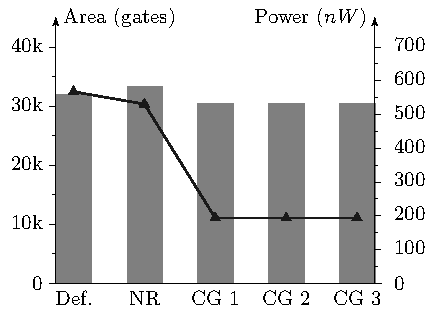
\includegraphics[width=8cm]{results-m1}}
		\caption{Syntheseresultaten voor de basis implementatie met en zonder register optimalisaties\label{figuur-resultaten-m1}}
\end{figure}

\section{Meerdere MALU's\label{sectie-resulaten-malus}}

Mits de toevoeging van extra MALU's is het mogelijk de totale rekeningtijd drastisch te verlagen (zie \refsect{subsectie-implementatie-gf2m-versnelling}). Hoewel het gebruik van meerdere MALU's de uiteindelijke schakeling vergroot en dat dus enigszins in gaat tegen de originele doelstelling, wordt hier toch onderzocht in welke mate de interessante parameters hierdoor juist worden be\"invloed. Er kan dan een afweging gemaakt worden tussen het gebruik van een schakeling met \'e\'en MALU op hogere kloksnelheid versus \'e\'en met meerdere MALU's aan een lagere kloksnelheid. De eerste schakeling zal kleiner zijn, maar waarschijnlijk wel meer verbruiken dan de tweede.

De totale berekeningstijd $t = \frac{c}{f}$ kan bepaald worden in functie van het aantal benodigde klokcycli $c$ en het aantal MALU's $d$:
\[c = 27058 + 2993 \cdot \left\lceil \frac{163}{d} \right\rceil,\]
waarbij 2993 het aantal vermenigvuldigingen is dat dient uitgevoerd te worden en de tweede term in de vermenigvuldiging het aantal klokcycli is dat een vermenigvuldiging kost. In \reftbl{tabel-resultaten-multi-cycles} wordt voor enkele waarden getoond hoeveel klokcycli nodig zijn om een berekening te voltooien. In \reffig{figuur-resultaten-multi-cycles} wordt hetzelfde weergegeven, maar dan voor elke $d$ van 1 t.e.m.\ 163. Het is duidelijk dat de tijdsbesparing waar extra MALU's voor zorgen vrij snel teniet wordt gedaan door het aantal cycli dat niet door $d$ be\"invloed wordt.

\begin{table}[h]
	\caption{Aantal klokcycli $c$ nodig voor \'e\'en pairing i.f.v.\ aantal MALU's $d$}
	\label{tabel-resultaten-multi-cycles}

	\centering
	\begin{tabular}{|l|l|l|l|l|l|l|l|l|}
		\hline
		$d$	& 1	& 2	& 3	& 4	& 6	& 8	& 16	& 32\\
		\hline
		$c$	& $514\:917$	& $272\:484$	& $191\:673$	& $149\:771$	& $110\:862$	& $89\:911$	& $59\:981$	& $45\:016$\\
		\hline		
	\end{tabular}
\end{table}

\begin{figure}[h]
	\centering
		\fbox{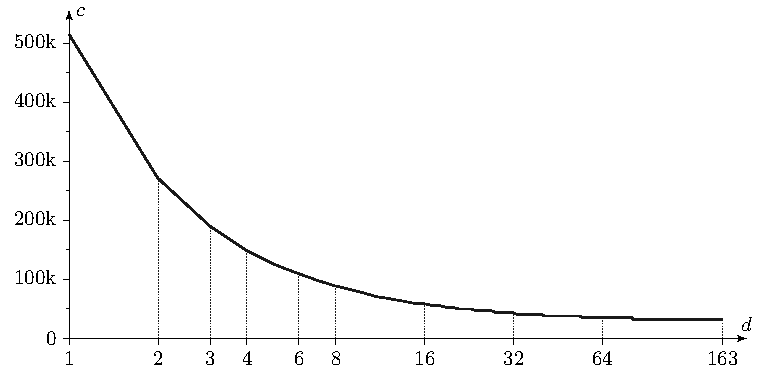
\includegraphics[width=\textwidth]{results-multi-cycles}}
		\caption{Aantal klokcycli $c$ nodig voor \'e\'en pairing i.f.v.\ aantal MALU's $d$\label{figuur-resultaten-multi-cycles}}
\end{figure}
      % Resultaten vd implementatie
\Chapter{Conclusie \& toekomstig onderzoek}

\section{Conclusie}

Deze thesis handelde over pairings, een recente ontwikkeling op gebied van cryptografie die identiteits-gebaseerde cryptografie toelaat. Er werd onderzocht hoe de Tate pairing ge\"implementeerd kan worden in hardware. Meer specifiek werd de nadruk gelegd op een compacte implementatie die daarbovenop nog eens zo weinig mogelijk vermogen verbruikte. Een implementatie van dat type zou toegepast kunnen worden in netwerken van sensoren of toestellen met een beperkt vermogen.

Verscheidene bestaande algoritmen werden aangepast en geoptimaliseerd zodat ze met een minimum gebruik aan geheugen uitgevoerd konden worden. Er werd een geheugenontwerp voorgesteld dat een goed compromis gaf tussen grootte en verbruik. Tevens werden verschillende oppervlakte- en vermogensbesparende technieken toegepast om het uiteindelijke circuit zo goed mogelijk aan de doelstellingen te laten voldoen. Door aanpassing van de kloksnelheid en het aantal gebruikte rekenschakelingen (MALUs) kunnen de parameters van het ontwerp aangepast worden aan de individuele normen van een toepassing.

Het resulterende ontwerp is uniek in zijn soort. Het verbruik per oppervlakte (genormaliseerd voor de werkfrequentie) van het gepresenteerde ontwerp is zeer laag. Ten tijde van dit schrijven waren nog geen andere ontwerpen gepubliceerd waarbij de nadruk op compactheid en laag vermogenverbruik lag.

\section{Toekomstig onderzoek}

Als toekomstig onderzoek kan het interessant zijn te onderzoeken of het mogelijk is het ontwerp nog verder te optimaliseren. Daarbij is het waarschijnlijk nuttig te trachten de gebruikte FSM verder te vereenvoudingen, aangezien die zowat de helft van de oppervlakte van de totale implementatie inneemt.

Verder zou ook onderzocht moeten worden in welke mate het werken over een groter Galois veld de oppervlakte en het verbruik wijzigt. Ook de implementatie van andere types pairings kan interessant zijn. Zo bestaan er bijvoorbeeld de $\eta_T$ en de modified Tate pairing die beiden berekend kunnen worden in ongeveer de helft van de tijd nodig voor de berekening van de Tate pairing.
       % Conclusie

\appendix                 % Start appendices

%\Chapter{GEZEL Code}            % Implementatie code
%\include{debugging}       % Manier van debugging

% BibTex referenties
%\cleardoublepage
\addcontentsline{toc}{chapter}{Bibliografie}
\bibliography{references}


% Lege achterpagina
%\clearpage
%\mbox{~}
%\thispagestyle{empty}

\end{document}
